\documentclass[final,3p,times]{elsarticle}
\usepackage[T1]{fontenc}
\usepackage{lmodern,amsmath,amssymb,amsthm,booktabs,graphicx,microtype,tabularx,placeins,float}
\usepackage[colorlinks=true,linkcolor=black,citecolor=black,urlcolor=blue]{hyperref}
\newtheorem{theorem}{Theorem}
\newtheorem{proposition}[theorem]{Proposition}
\setlength{\emergencystretch}{2em}
\renewcommand{\topfraction}{.93}\renewcommand{\textfraction}{.07}\renewcommand{\floatpagefraction}{.75}
\graphicspath{{figures/}}
\journal{Advanced Engineering Informatics}
\begin{document}
\begin{frontmatter}
\title{Executable Operating Contracts Linking Anytime Localization to Engineering Task Evidence}
\author[ae]{Chuansu Peng}
\author[ae]{Haoran Dong}
\author[ae]{Ruoxuan Wu}
\author[etc]{Peipei Zeng}
\address[ae]{School of Aeronautical Engineering, Civil Aviation University of China, China}
\address[etc]{Engineering Training Center, Civil Aviation University of China, China}
\begin{abstract}
Aircraft inspection requires a timely airframe-relative pose and evidence matched to the consuming task. We develop executable operating contracts linking pre-sensing event requirements, computation budgets, source-version execution and population-risk applicability. Typed dependencies select compatible frozen policies, constrain refinement/publication and revoke source-scoped statements after detected invalid attempts while preserving valid numerical installation. A prospective study uses 13,824 synthetic episode inputs, 22 matched policies, 4,096 independent confirmation inputs and 432 live complete-route executions. Exact finite-family calibration treats trajectory, observation and their union separately. At standard service the retained CART policy reduces integrated error loss versus Fixed2 by 15.68\% on nominal geometry and 12.61\% on unfitted geometry, with higher modeled work. Matched FlatCART gives identical numerical results; a fully validated task-aware procedural baseline matches the complete contract service. History enforcement removes all incorrect attachments in 16 constructed invalid cases, also achieved by that strong procedural baseline. At risk allowance 0.15, 18 of 32 configured requests are feasible; tight-service and unsupported-route evidence is refused. Ordinary routes can favour Fixed2, and one contended certificate has only 0.00367 margin. The contribution is an executable, auditable task--source--evidence interface, with service-dependent numerical trade-offs, rather than a universal accuracy gain or physical safety guarantee. No new physical localization experiment is reported.

\end{abstract}
\begin{keyword}
Executable operating contracts \sep Engineering decision knowledge \sep Anytime localization \sep Evidence applicability \sep Risk calibration \sep Aircraft inspection
\end{keyword}
\end{frontmatter}
\section{Introduction}\label{sec:introduction}
An aircraft-inspection system needs more than a low-error pose. An observation must receive a fresh airframe-relative correction before its deadline; a continuing route needs acceptable error over a longer interval. The same localization computation can satisfy one requirement and fail the other. Moreover, a reliability statement established for one registration policy, sensor mixture or installation service does not automatically apply after a software update or a revision of the pose. The engineering decision is therefore which computation to execute, when to expose its result, and which evidence remains applicable to the result that a task actually consumes.

This problem connects engineering decision knowledge to an executable numerical service. Work on process and decision knowledge representation shows how explicit dependencies support engineering decisions \cite{wang2021process,hao2021knowledge,su2025manufacturing}. Contract-based design makes assumptions and guarantees part of a component interface \cite{benveniste2018contracts}. Anytime autonomous systems already connect computational contracts to estimation and control \cite{pant2021}; perception scheduling also studies the tradeoff between latency and precision \cite{aldana2023}. The unresolved issue addressed here is narrower: an interrupted registration produces correlated revisions of one source, whereas a population-risk statement refers to a complete policy, installation model and specified task event. Their identities and lifetimes must remain consistent from pre-sensing selection to installed pose and final evidence attachment.

Our previous A19/A20 development established retained registration prefixes, source-time replacement and empirical computation--error tradeoffs. It also exposed three limitations. A guarded CART scheduler often behaved like its flat predictor; fixed two-iteration registration could outperform it on ordinary complete routes; and metadata prototypes did not establish an integrated evidence lifecycle. Increasing a favorable mean or adding a knowledge-labelled diagram would not resolve these limitations. We retain the estimator and assets and instead test the contract mechanism against a task-aware, risk-calibrated procedural implementation supplied with the same information.

We represent sources, versions, policies, operating profiles, processing services, requests and calibrated event cards as typed entities with explicit dependencies and execution predicates. A task declared before sensing selects an admissible frozen policy or receives a refusal. During execution, budget and predicted-time constraints restrict computation, correlated results replace the same source posterior, and measured motion is replayed to installation. A source-scoped attachment monitor checks the identity and history needed to associate the installed result with its population-risk statement. Changes to a dependency revoke affected claims. A numerical result can remain available with a provisional status after its statistical attachment becomes inapplicable.

The study makes three contributions.
\begin{enumerate}
\item An executable representation of the relationship between engineering requirements, numerical versions and statistical evidence, including pre-sensing policy commitment, selective dependency invalidation and permanent source-level attachment refusal after a detected invalid version attempt. These mechanisms are evaluated separately from pose accuracy.
\item A common localization service that combines retained ICP computation, constrained publication, source replacement and causal replay. A dimensionally consistent work objective and two explicit timing ledgers permit comparisons with fixed, learned and earlier RAVC policies under the same resources.
\item A prospectively frozen empirical assessment of contract modules, task-driven selection, directly calibrated union events, certificate margin, unfitted geometry, binding time/profile constraints, continuous routes and influential failures. A fully validated procedural comparator prevents the engineering representation from receiving credit for information or checks withheld from its baseline.
\end{enumerate}

The central hypothesis is that executable knowledge can prevent an engineering task from using evidence outside its scope while making computational tradeoffs explicit. It does not require graph storage to outperform a semantically equivalent program in localization accuracy. We accordingly separate numerical localization, engineering decision quality and evidence-attachment correctness. The new experiments use simulated geometric sensors and a declared processing model; original platform photographs and previous studies remain as documented context. No new physical localization experiment is claimed.

Figure~\ref{fig:contracts} follows the complete decision path. Sections~\ref{sec:problem}--\ref{sec:method} define its objects, rules and execution. Section~\ref{sec:theory} states the properties needed to justify replacement and evidence applicability. The prospective protocol and results in Sections~\ref{sec:design}--\ref{sec:evaluation} distinguish independent inputs from repeated method executions and retain unfavorable fixed-policy results.
\begin{figure}[t]\centering
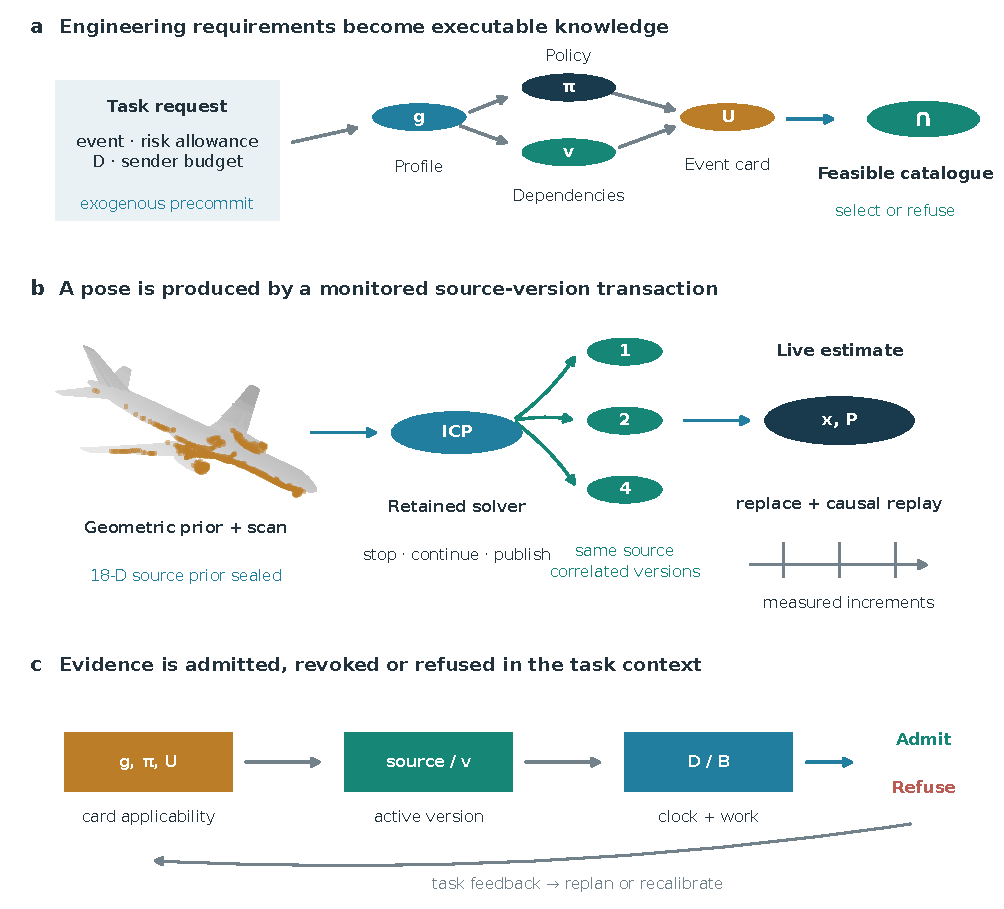
\includegraphics[width=\linewidth]{r8/architecture.pdf}
\caption{Executable engineering requirements, numerical execution and evidence applicability. (a) An exogenous event requirement, risk allowance, deadline and budget constrain a dependency-bound policy catalogue. (b) Retained computation revises one immutable source; ordered replacement and measured-motion replay produce the live pose. The airframe surface and source points illustrate an actual excluded pilot input. (c) Final attachment checks join an event card to the active source version and its service; invalid history or dependencies remove the bound. The feedback arrow denotes the interface for a future request or recalibration; autonomous feedback replanning and a physical control experiment are not evaluated. OpenAI ChatGPT/Codex (GPT-6) assisted the archived Python schematic code.}\label{fig:contracts}
\end{figure}

\section{Related work and contribution boundary}\label{sec:related}
\paragraph{Engineering knowledge and executable contracts.}
Process knowledge representation links decision context, alternatives and dependencies in complex engineered systems \cite{wang2021process}. Decision knowledge graphs integrate and navigate engineering decisions \cite{hao2021knowledge}; manufacturing work further uses graph learning for knowledge reasoning \cite{su2025manufacturing}. Our representation is a typed dependency graph and a monitored state machine. It performs deterministic applicability checks, selection and invalidation. It does not learn relations or claim general semantic reasoning. Contract theory provides a much broader algebra of assumptions, guarantees and composition \cite{benveniste2018contracts}. We implement a specific operating contract whose statistical part concerns a fixed policy and an explicitly defined localization event.

\paragraph{Computational decisions in autonomous systems.}
Metareasoning and anytime algorithms treat computation as a decision with opportunity cost \cite{russell1991meta,zilberstein1996anytime,hay2012}. Pant et al. already use contract-driven anytime estimation and control with robust model-predictive control and a physical aerial platform \cite{pant2021}. Their work is the closest precedent for connecting computational contracts to autonomy. We do not claim the first such connection, robust closed-loop control or a new general optimal-stopping theorem. Perception scheduling can preserve stability while trading latency against precision \cite{aldana2023}; computational abstraction relates robot task accuracy to compute expenditure \cite{ghosh2021}; kernel studies characterize practical computational demand \cite{sifat2023}. Here the distinctive execution object is a correlated source-version stream, and the evidence object is an event-specific, population-level risk card that must retain that stream's policy and installation identity.

\paragraph{Registration and state consistency.}
ICP variants and point-cloud registration are established methods \cite{besl1992icp,chen1992,segal2009gicp,pomerleau2015}. Our contribution lies in exposing a retained solve and governing its publication, not in replacing the registration objective. ICP curvature is also an imperfect surrogate for error uncertainty \cite{censi2007,bonnabel2016,brossard2020}. We therefore retain the joint robot/map state, propagate its covariance, and obtain empirical risk bounds from entire executed episodes rather than interpreting a Hessian as calibrated confidence. Delayed-measurement estimation already addresses temporal consistency \cite{barshalom2002}; our immutable-source replacement handles correlated revisions of one solve rather than fusing them as independent observations. Complete localization systems such as KISS-ICP and FAST-LIO2 address broader odometry and mapping problems \cite{kiss2023,xu2022}. They are not substituted for same-task scheduling controls: our task uses a supplied structural prior and a common scan registration interface.

\paragraph{Risk control and runtime assurance.}
Exact binomial inversion supplies the one-sided confidence bounds \cite{clopper1934}. Learn-then-test separates fitted predictive algorithms from risk-controlled selection \cite{angelopoulos2025ltt}; conformal risk control and conformal policy control provide other principled control constructions \cite{angelopoulos2024crc,prinster2026}. We use a finite, pre-frozen catalogue with Bonferroni allocation because the events are binary and simultaneous bounds directly support the requested selector. This is not a new statistical bound. Runtime-assurance architectures can switch to a safety controller \cite{mehmood2022simplex}; our refusal withdraws statistical attachment or retains an uncorrected pose and supplies no physical safety guarantee. The engineering contribution is the executable correspondence between requirements, numerical execution and evidence lifetime, assessed against an independently coded procedure that can enforce the same semantics.

\begin{table}[t]\centering\footnotesize
\caption{Closest mechanism precedents and the object evaluated here. The rows describe supported research objects and do not assert that a precedent lacks every other capability.}\label{tab:mechanism-precedents}
\begin{tabularx}{\linewidth}{@{}p{.20\linewidth}XXX@{}}\toprule
Study & Research object & Decision and conditions & Evaluation or claim boundary\\\midrule
Contract theory \cite{benveniste2018contracts} & Assumption--guarantee specifications and their composition & Component compatibility under stated assumptions & General design formalism; not a new algebra in this paper\\
Pant et al. \cite{pant2021} & Error/delay contracts for anytime estimation and control & Joint computation/control with robust MPC conditions & Physical aerial-platform and closed-loop control evaluation\\
Learn-then-test \cite{angelopoulos2025ltt} & Risk-controlled predictive configurations & Multiple tests admit configurations from calibration & Statistical risk control; used as an established selection principle\\
Runtime assurance \cite{mehmood2022simplex} & Safe autonomy with a fallback controller & Monitoring and switching under safety conditions & Control assurance; our evidence refusal supplies no physical safety theorem\\
This study & Correlated pose revisions and event evidence bound to their policy/source/installation identity & Pre-sensing commitment, compatible execution, source-scoped statement lifetime & Numerical, task and applicability endpoints tested separately against a complete procedural control\\\bottomrule
\end{tabularx}
\end{table}

\section{Localization service and engineering events}\label{sec:problem}
\subsection{Joint state and immutable source}
The robot localizes against a stationary airframe prior. The retained state is $x=(t,R,b,m_t,m_R)$, with translation, rotation, six motion-bias components and map translation/rotation. Its covariance $P$ spans an 18-dimensional local perturbation. Reported airframe-relative position error is
\begin{equation}
e_p=\widehat m_R^\top(\widehat t-\widehat m_t)-(m_R^\star)^\top(t^\star-m_t^\star).
\label{eq:relative-error}
\end{equation}
Measured motion increments propagate the joint state and covariance through $x_{k+1}=f(x_k,u_k)$ and $P_{k+1}=F_kP_kF_k^\top+Q_k$, using an $SE(3)$ local linearization \cite{barfoot2014}. Bias follows a first-order Gauss--Markov model. Truth is available to the simulator and scorer, not to the online policy or contract checker.

A source $s$ comprises a scan and an immutable source-time prior $(x_s^-,P_s^-)$. Registration checkpoint $j$ exposes candidate $(x_s^{(j)},P_s^{(j)})$, causal features $h_j$ and cumulative work. These candidates revise one likelihood evaluation against the same prior. On delivery at $t_d$, the receiver assigns
\begin{equation}
(x_{t_d}^{(j)},P_{t_d}^{(j)})=\mathcal R_{s\to t_d}(x_s^{(j)},P_s^{(j)};u_{s+1:t_d}).\label{eq:replay}
\end{equation}
The measured increments are replayed only to a time already acquired. Later candidates replace earlier source versions; they are not fused as independent measurements. A rejected completion after a transient publication emits the original source prior as an ordered rollback. The service admits one active source job. A job releases its slot after its computation and all pending publications, including rollback, have drained. Interleaved independent measurements would require rewind and reprocessing and are outside this serial interface.

\subsection{Three explicit event requirements}
For an episode of duration $T=4$~s, the loss is $L_\pi=\int_0^T\|e_p^\pi(t)\|^2dt$, reported as the right-endpoint sum $\widehat L_\pi=0.1\sum_{k=1}^{40}\|e_p^\pi(0.1k)\|^2$. The trajectory event is
\begin{equation}
E_{\rm tr}=\{\max_{t\in\{0.5,0.6,\ldots,4.0\}}\|e_p(t)\|>\epsilon\},\qquad\epsilon=0.10\ {\rm m}.\label{eq:episode-event}
\end{equation}
The first 0.5~s remains part of the reported loss and is identifiable as startup exposure. For an observation deadline $D$, define
\begin{equation}
E_{\rm obs}=\{\text{no positive scan version is active at }D\}\cup\{\|e_p(D)\|>\epsilon\},\qquad
E_{\rm un}=E_{\rm tr}\cup E_{\rm obs}.\label{eq:observation-event}
\end{equation}
Same-tick ordered installation and rollback precede assessment. A superseded positive version does not count as ready. The observation event is a correction-availability/position proxy; it does not model camera orientation, image quality or defect detection. The 0.10-m threshold is a study metric, not an aircraft clearance standard.

A request may require trajectory, observation, both \emph{marginal} bounds, or a directly calibrated union bound. These four requirements differ: $U_{\rm tr}\le\delta$ and $U_{\rm obs}\le\delta$ imply only a union bound of $\min(1,U_{\rm tr}+U_{\rm obs})$. A union request instead uses the binary event $E_{\rm un}$ in calibration.

\subsection{Work, deadlines and measurement boundaries}
We keep two ledgers. The deterministic operation clock assigns CPU-equivalent seconds to actual counted registration queries, checkpoints, forecast traversals, publication/checking, front-end processing and propagation. Its coefficients are characterized on 48 excluded pilot inputs and frozen before calibration. This clock defines the controlled experiment's sender budget and installation schedule. Separately, native process CPU records work that actually executed. Controlled comparisons charge the shared executed front end, solver prefix, forecast and odometry to each policy; integrated wrappers additionally time their measured claim bookkeeping and receiver components. Complete routes time the entire live online loop. Raycasting, file decompression and truth scoring are offline costs.

The hard stage budget $B$ covers source sealing, registration, features, forecasts, rules and publication witnesses. It excludes the common front end and receiver/stream work, which remain included in total work and availability. A common conservative stage reservation prevents every policy, including a fixed cap, from starting unaffordable registration work. Thus an effective Fixed2 service may stop before two iterations when its budget binds; its newly calibrated card refers to that complete wrapper.

For publication $j$, let $c_j$ be total sender work including the front end, $r_{<j}$ accumulated receiver work, $h$ propagation work per step and $r_0$ fixed receiver work. Queue delay is $q=0.05$~s and $\Delta t=0.1$~s. The controlled installation rule is
\begin{equation}
n_j=\max\left(1,\left\lceil\frac{q+\alpha(c_j+r_{<j}+r_0)}{\Delta t-\alpha h}\right\rceil\right),\qquad
r_{<j+1}=r_{<j}+r_0+n_jh.\label{eq:delivery}
\end{equation}
The denominator is positive in the frozen services. Complete routes execute causal incremental replay and defer installation until the modeled work is available. The load factor $\alpha$ represents constructed contention. Neither clock characterization nor $\alpha$ is an embedded-device latency measurement or a worst-case execution-time guarantee.

Selection minimizes $\overline L_\pi+\lambda_{\rm sel}\overline W_\pi$, with $\lambda_{\rm sel}=1$~m$^2$ and $W$ in CPU-equivalent seconds. The objective has units m$^2$s. Native CPU is reported separately and never added to loss without a stated weight.

The controlled-prefix ledger sums measured native component CPU. A second ledger times the inclusive replay program and includes offline truth assertions and scoring; it is reported separately and is not presented as pure online service CPU. Complete-route experiments directly time the online computation loop with sensor raycasting, archive decompression and truth scoring outside that boundary.

\section{Executable knowledge, constraints and evidence}\label{sec:knowledge}
\subsection{Typed representation and applicability}
Define the operating knowledge structure as
\begin{equation}
\mathcal K=(\mathcal V,\tau,\mathcal R,\sigma,\Gamma),\label{eq:knowledge-record}
\end{equation}
where $\mathcal V$ contains entities, $\tau$ assigns their types, $\mathcal R$ contains typed relations, $\sigma$ stores immutable specifications and fingerprints, and $\Gamma$ contains executable predicates. Types are Source, Version, Profile, Service, Policy, Predictor, EventCard and Request. The dependency subgraph is directed and acyclic; ordered revision is maintained by the source transaction. This concrete representation uses dictionaries, a dependency graph and monitored state, without an ontology language or learned knowledge-graph embedding.

\begin{table}[t]\centering\small
\caption{Knowledge entities, executable conditions and consequential decisions.}\label{tab:knowledge}
\begin{tabularx}{\linewidth}{@{}lXX@{}}\toprule
Entity/relation & Stored information and condition & Execution or evidence consequence\\\midrule
Source; derived-from & Scan fingerprint; all source-prior state and covariance arrays sealed & Revisions must use the same source and prior\\
Version; revises & Producer-recorded sequence, iteration, payload seal and rollback flag & Ordered replacement; no resurrection after rollback\\
Profile; applicable-under & Whole sampling mixture and geometric artifact & Restrict refinement; refuse unmatched population evidence\\
Service; executes-with & Queue, load, deadline, budget, clock and same-tick order & Reserve sender work; compute receiver availability\\
Policy/Predictor; depends-on & Frozen rule specification, model and implementation hashes & Admit the executed policy; invalidate affected cards after change\\
EventCard; supports & Defined event, $n,k,K,\beta,U$, calibrated profile/service & Select only admissible event requirements\\
Request; authorized-by & Pre-sensing task, finite allowance and selected-card seals & Commit a policy; attach a matching population statement or refuse\\\bottomrule
\end{tabularx}
\end{table}

The representation distinguishes three epistemic roles. Correspondence counts, residuals and motion increments are measured observations. Sensor noise settings, geometric identity and service parameters are declared configurations. Equality of deployment and calibration distributions is an assumption. A metadata match checks the second role; it cannot establish the third or detect hidden distribution shift.

A card is $c=(g,a,\pi,e,n,k,K,\beta,U,\nu)$, where $g$ is a complete population profile, $a$ a processing service, $\pi$ a complete effective policy, $e$ an event and $\nu$ its version dependencies. Schema validation checks finite values, integer counts, exact binomial inversion and the body fingerprint before admitting a card to the trusted registry. Dependencies include the relevant predictor, policy specification, solver, executor, contract implementation, event definition, service, profile, protocol and geometric artifacts. Predictor changes invalidate only dependent policies; global clock changes invalidate every card. Fingerprints identify artifact equality in this controlled software setting; they do not provide remote device attestation or cryptographic authentication against a compromised producer.

\subsection{Exogenous task selection and commitment}\label{sec:dispatch}
A request $R=(g,a,\mathcal E,\delta)$ is declared before its scan is opened. The service specifies $D,B,\alpha$; $\mathcal E$ is one event or the two marginal events. With frozen catalogue $\Pi_0$, define
\begin{equation}
\Pi(R)=\{\pi\in\Pi_0:\operatorname{match}(g,a,\pi,\nu)\ \land\ U_{g,a,\pi,e}\le\delta\text{ for every }e\in\mathcal E\}.\label{eq:dispatch-set}
\end{equation}
The selector chooses
\begin{equation}
\pi^*(R)=\arg\min_{\pi\in\Pi(R)}(\overline L_{g,a,\pi}+\lambda_{\rm sel}\overline W_{g,a,\pi}),\label{eq:dispatch-choice}
\end{equation}
with policy-ID tie-breaking. Empty sets return \texttt{REFUSED}. Calibration estimates may determine the choice because all bounds are simultaneous. No scan quality, confirmation outcome or future error enters selection. The selected policy remains fixed across its declared population; per-scan switching between calibrated policies would define a different policy needing its own calibration.

The selector emits a witness containing the request, chosen policy, card seals, event bounds and active dependency snapshot. A trusted precommit copies it before source acquisition. Binding the actual source changes its phase from \texttt{PRECOMMITTED} to \texttt{SOURCE\_BOUND}; subsequent request or policy replacement is rejected. A new task requires a new exogenous commitment. This rule prevents a bound for one population-level policy from being attached to a favorable scan-selected alternative.

\subsection{Action constraints and lifecycle enforcement}
Time and profile constraints affect the numerical candidate set. The time predicate removes forecast caps whose estimated availability exceeds $D$. It accounts for the new candidate's own replay but omits previously accumulated receiver work; remaining solve cost is also a conditional mean. It is therefore an optimistic screen rather than a deadline guarantee. The executed installation rule in Eq.~\eqref{eq:delivery} includes accumulated receiver work, and event calibration uses that actual modeled installation. The profile predicate caps refinement at four iterations when declared noise exceeds two, source position standard deviation exceeds 0.061~m, or the geometry was excluded from predictor fitting. Both predicates were fixed on development evidence. They provide bounded fallback behavior, not a proof that mismatch has been detected or corrected. The common hard-budget reservation applies to every policy independently of these two predicates.

Each produced version is registered by the trusted producer with its sequence, iteration, rollback flag and payload seal. Before installation, the receiver checks the source/prior/data identities, current dependency values, committed policy, configuration, producer record, sequence and iteration order, rollback semantics, causal replay time, finite clock and sender work. Checking both the incoming payload and the producer record prevents jointly rewriting a payload and its advertised checksum in the tested trust model. A rejected packet is not installed. A valid late numerical correction may still install after an observation deadline, but its observation statement is expired.

Statistical attachment is an additional operation. It requires the matching requested event and card, current source/version/payload, assessment instant, allowable risk and active dependencies. The attachment identifies an unconditional \emph{policy/population event bound}; it is not a confidence score for this pose. An installed rollback remains part of the policy's calibrated behavior and is not itself a malformed-history fault.

The source-scoped history monitor addresses a lifecycle gap: a valid later packet must not restore a statement after an invalid attempt has changed the execution's evidence status. Scope state persists across ledger/plan reconstruction within the trusted registry's lifetime; process restart requires restoring that state or withholding attachment. For trusted source-execution scope $s$, it maintains
\begin{equation}
M_{s,0}=1,\qquad M_{s,j+1}=M_{s,j}\land C_{s,j},\qquad
A^{\rm issued}_{s,j}=A^{\rm candidate}_{s,j}\land M_{s,j+1},\label{eq:history-latch}
\end{equation}
Here $C$ is the original operational receiver check. Every receipt reads the updated latch after that check; earlier receipt objects in the trusted ledger are marked revoked. This is local service state, not a claim of network revocation notification. The full representation revokes a source-specific claim child of the reusable plan; the procedural comparator independently maintains a monotone Boolean. Earlier receipts receive revocation records, and later receipts return \texttt{PROVISIONAL} with an empty upper bound. The operational plan is preserved, so later valid numerical installation is unaffected. Scope comes from the trusted execution context, even if a packet falsely names another source. Ordinary admission refusal and scheduled statement expiry do not trip this latch.

This monitor detects the specified invalid attempts. It does not detect an unobserved missing packet, an undeclared physical change or a malicious trusted producer. Such conditions lie outside the canonical execution/population assumptions. The monitor was sealed as an explicitly disclosed attachment amendment after numerical freeze F0 and before selection freeze F1; it preserves the numerical clock and event map (Section~\ref{sec:theory}). Its actual CPU is measured rather than claimed to have been characterized by the earlier pilot fit.

\subsection{Task feedback and a fair procedural alternative}
The service returns a numerical pose plus readiness and one of attached, provisional or refused evidence states. A consumer can request a different deadline/budget, wait for a new exogenous source, or initiate offline recalibration for a changed profile. It cannot manufacture a valid certificate by relabelling metadata. In complete-route experiments, the population is deliberately distinct: admission refuses episode evidence and the service continues explicitly provisional localization with a descriptive nearest-profile recommendation.

The strongest comparator, \texttt{TaskAwareFlatValidated}, has the same catalogue, calibration costs, event requirements, risk allowances, budgets, precommit, source information and producer records. Its independently coded conjunction implements all current-version and history checks without the dependency graph. Equivalence is a meaningful outcome: it would show that executable semantics, rather than graph storage alone, cause the effect. We also test stripped checks as mechanism ablations, clearly separated from this fair competitor. Numerical accuracy, task feasibility and incorrect evidence attachment therefore have distinct denominators and conclusions.

\section{Retained numerical execution and calibrated policy family}\label{sec:method}
\subsection{Registration and correlated checkpoints}
We preserve the A19/A20 robust point-to-plane solve against a fixed source prior. For $d=x\boxminus x_s^-$,
\begin{equation}
\Phi_s(x)=d^\top(P_s^-)^{-1}d+\sigma^{-2}\left[\sum_{i\in\mathcal I(x)}\rho(r_i(x))+(n-|\mathcal I(x)|)\rho(r_{\rm out})\right].\label{eq:objective}
\end{equation}
Huber scale is 0.0625~m, $\sigma=0.025$~m and unmatched residual $r_{\rm out}=0.8$~m. The unmatched term prevents improvement by discarding difficult correspondences. The solve uses at most 96 deterministically thinned points and 25 iterations, with backtracking fractions $1,1/2,1/4,1/8,1/16$. Checkpoints occur at iterations $1,2,4,8,16,25$ or termination. Each curvature covariance is constructed from the same prior precision,
\begin{equation}
P_s^{(j)}=\operatorname{PSD}\left[(G_j^\top(P_s^-)^{-1}G_j+H_j^\top\Omega_jH_j)^{-1}\right],\label{eq:checkpoint-cov}
\end{equation}
including rotation perturbation Jacobians. It is a local curvature approximation, not an empirically calibrated error covariance.

An eligible candidate requires a descending step, at least 12 pairs, clipped residual RMS below 0.065~m and more than 60\% of residuals within 0.10~m. Final acceptance additionally requires translation and orientation steps below 0.001~m and 0.0005~rad. An interrupted eligible candidate may be published without final convergence. Continuation retains the iterate, prior precision and computational prefix. A final rejection after transient publication restores the original source prior through the same version/replay interface.

\subsection{Common predictors and module interventions}
The retained CART and random forest use the same 1,120 source-grouped development inputs, with 926 training and 194 validation sources. They are not refitted in this revision. CART has depth seven and minimum leaf size 20; the forest averages 64 depth-eight trees with minimum leaf size 12. Inputs are causal prior uncertainty, weakest scaled pose-information eigenvalue, residual/inlier measures, step sizes, objective ratio, iteration, pair count, displacement and declared noise. Aircraft identity, source truth, future motion and true error are excluded.

For reachable cap $a\in\{2,4,8,16,25\}$, the predictor supplies terminal MSE $\widehat v_{ja}$, development trajectory-event frequency $\widehat r_{ja}$ and remaining work $\widehat c_{ja}$. Current-candidate and source-prior MSE predictions govern publication. Effective terminal labels account for ineligible/rejected completion and prior rollback. The endpoint forecasts are heuristic; their event frequencies are not risk certificates. With constrained candidate set $\mathcal A_j$,
\begin{equation}
\widehat a_j=\arg\min_{a\in\mathcal A_j}
\{T\max(\widehat v_{ja},0)+\lambda\max(\widehat c_{ja},0)+\omega\operatorname{clip}(\widehat r_{ja},0,1)\},\label{eq:stop-rule}
\end{equation}
where $\lambda\in\{0.3,1,3\}$~m$^2$ and $\omega=0.002$~m$^2$s. Forecast work retains its native development-label scale as a mean proxy; actual experiment availability and risk labels use the frozen operation clock. Matched variants use exactly the same forecasts and prices. At iteration two or later, selection of an already reached cap stops the job. Empty deadline-feasible sets and the profile cap may also stop it. Eligible interim candidates publish when their predicted MSE improves on the prior; eligible interrupted terminal candidates publish as well.

The 22-policy catalogue contains contract-CART (KG), FlatCART, FlatRF and ContractRF at all three prices; Fixed2, Fixed4, Fixed8, Fixed16, Final, Residual, seeded Random2or4 and OldRAVC; and price-one CART/RF time-only interventions. The name KG is retained for trace continuity, without implying a learned knowledge-graph model. Flat predictors omit time/profile guards; time-only variants add only time; KG/ContractRF add time and profile. Evidence-match and full-lifecycle layers then operate on the same numerical trace. This sequence distinguishes action changes from statement changes. All methods receive the common budget wrapper, inputs, service and acquisition/replay semantics.

OldRAVC retains the earlier six-output CART (480 training/120 validation inputs, depth six). It forecasts current/final MSE, their trajectory-event frequencies, remaining CPU and current-minus-prior MSE. An eligible candidate publishes if its forecast event frequency is at most 0.30 and its predicted MSE improves on the prior. From iteration two, an eligible candidate stops and publishes if its forecast event frequency is at most 0.30 and its predicted four-second MSE gain is no greater than remaining-work cost with price 1~m$^2$. Final acceptance follows the common solver. Unlike the new CART/RF features, this legacy model retains the binary C172 identity feature; the unfitted geometry uses the non-C172 value. Residual publishes an eligible checkpoint and stops at the first eligible checkpoint from iteration two. Random2or4 chooses cap four with frozen development continuation probability 0.4654427646, otherwise cap two, using a deterministic SHA-256 seed coin. Fixed caps publish an eligible reached cap, whereas Final waits for solver termination. Budget interruption can alter each nominal cap.

\subsection{Exact finite-family calibration}
For each fixed profile, service, policy and event, $k$ of $n$ independent input seeds produce failures. With $\beta=0.05$ and
\begin{equation}
K=22\times2\times4\times3=528,\qquad
U=\begin{cases}1,&k=n,\\\operatorname{Beta}^{-1}(1-\beta/K;k+1,n-k),&k<n,\end{cases}\label{eq:cp}
\end{equation}
we store one card per combination. Trajectory, observation and union use their own binary counts on the same input, without multiplying the independent sample size. There are 4,096 calibration seeds per profile. Same-input correlations across methods, services and events are permitted by the simultaneous argument.

All 96 profile/service/task/allowance requests are selected and sealed at F1 before confirmation generation. Requiring both marginals checks two cards; requiring union checks its directly calibrated card. The primary allowance is 0.15; 0.10 and 0.20 describe a frozen feasibility grid. Prefix sample-size and confidence analyses diagnose margin sensitivity and do not change a deployed plan. A card with a barely positive margin remains admissible but is reported as fragile rather than described as robust.

\begin{table}[t]\centering\small
\caption{One guarded source execution. All checks use causal inputs or declared specifications.}\label{tab:algorithm}
\begin{tabularx}{\linewidth}{@{}rX@{}}\toprule
1 & Validate the exogenous task and select a feasible policy/card set; refuse an empty catalogue and retain the propagated prior.\\
2 & Precommit the plan, bind the actual scan and immutable joint prior, and register their seals.\\
3 & Reserve the next stage under the common budget; execute only its new ICP prefix and checkpoint features.\\
4 & Apply the matched predictor and time/profile predicates; stop, continue or produce a sealed candidate.\\
5 & Validate the received version against producer records and active dependencies; reject malformed attempts and latch the source's claim status.\\
6 & Replace the source version and replay acquired motion; include checking and replay in the execution ledgers.\\
7 & Issue only a matching, unexpired population-event receipt from the source-scoped attachment layer.\\
8 & Honor final rejection/rollback; report pose, readiness and evidence status to the task consumer.\\\bottomrule
\end{tabularx}
\end{table}

OpenAI ChatGPT/Codex (GPT-6, developer OpenAI) assisted research-program and plotting-code development, computational analysis and exact schematic code. Archived programs produce the numerical observations from the specified geometric inputs; the figure scripts regenerate data plots and source/version schematics. The release records the actual assistance and authors must review and accept responsibility for the final content before submission.

\section{Properties supporting the execution and evidence interface}\label{sec:theory}
The results below concern source consistency, exposure and the scope of a statistical statement. They do not assign an optimality guarantee to the learned endpoint heuristic. Earlier finite decision and scalar deployment models are retained in the supplement.

\begin{proposition}[Source replacement]\label{prop:version}
Assume all candidates of one source use its immutable scan/prior, publication leaves the retained solve unchanged, and no independent measurement update interleaves with the source job. Replacing an intermediate version with the final candidate and applying Eq.~\eqref{eq:replay} gives the same live state and covariance as delivering that final candidate alone at the same installation time. A final prior rollback has the same property.
\end{proposition}
\begin{proof}
The final candidate is the same deterministic function of scan, prior and executed prefix in both schedules. At final delivery both receivers assign the replay of that same candidate using the same acquired motion increments. The replay begins from the same covariance as well as state. No intermediate candidate contributes a second likelihood factor.
\end{proof}
The premise is why the receiver replaces a source instead of recursively fusing checkpoints. Cold-solve and live-prefix audits test the retained implementation; the property does not assert unbiased intermediate ICP error.

\begin{proposition}[Delivery exposure]\label{prop:exposure}
Consider two schedules with the same source candidates, exogenous motion and aligned final installation $\tau_f$. One publishes an intermediate candidate at $0\le\tau_c<\tau_f\le T$; the other holds it. If $e_0$ is the old-prior error and $e_c$ the replayed candidate error, then
\begin{equation}
\mathbb E[L_{\rm hold}-L_{\rm publish}]
=\int_0^T\mathbb E\!\left[\mathbf 1\{\tau_c\le t<\tau_f\}\big(\|e_0(t)\|^2-\|e_c(t)\|^2\big)\right]dt.\label{eq:exposure}
\end{equation}
\end{proposition}
\begin{proof}
Before $\tau_c$ the live estimates coincide, and after $\tau_f$ they coincide by Proposition~\ref{prop:version}. Subtract the loss integrals pathwise and exchange integration and expectation under integrability. Deterministic delivery times reduce the expression to an integral over $[\tau_c,\tau_f)$. For multiple publications, use the actual live candidate on each interval.
\end{proof}
An eligible residual alone does not determine the sign. Under linear propagation with common independent future noise, the difference contains the actual source error covariance and squared-mean differences; the curvature matrices need not equal those covariances. Publication also pays replay work. The experimental held-publication intervention recomputes timing after removing earlier replay and can change final installation, so its empirical contrast includes that additional effect.

\begin{theorem}[Simultaneous population-event bounds]\label{thm:calibration}
Freeze the $K$ profile/service/policy/event combinations independently of calibration outcomes. For each combination, assume independent, identically distributed complete calibration inputs from its stated deployment mixture, including any independent policy randomization, and keep its entire effective execution/event map fixed. With Eq.~\eqref{eq:cp}, probability at least $1-\beta$ over calibration gives $r_{g,a,\pi,e}\le U_{g,a,\pi,e}$ simultaneously for every combination. On this confidence event, any calibration-dependent selection from Eq.~\eqref{eq:dispatch-set} satisfies its requested population-event allowances.
\end{theorem}
\begin{proof}
A fixed combination has a binomial failure count. Exact one-sided inversion has undercoverage at most $\beta/K$. A union bound over the fixed combinations gives simultaneous coverage. On that event all bounds hold, including those of a policy selected using calibration cost and event counts. Independence across policies, services, events or sampled instants is unnecessary.
\end{proof}
The reproducible Random2or4 comparator obtains its cap from a seed hash. Its binomial interpretation assumes that the seed-derived coin is an independent draw in the complete-input model. Conditioning instead on a fixed heterogeneous cap assignment does not yield the same iid binomial model; that interpretation would require a different bound. All simulator random streams share the usual ideal independent pseudorandom-stream modeling assumption.

Confidence $1-\beta$ concerns uncertainty in population risk; $\delta$ concerns an episode event. The two probabilities differ. A union card calibrates $E_{\rm tr}\cup E_{\rm obs}$ directly and may differ from both marginal decisions. For $M$ deployment episodes, the generic mission bound is only $\min(1,M\delta)$ without further structure. Neither a route certificate nor subgroup/scan-conditional risk follows from an episode card. Declared configuration matching cannot replace the distribution assumption.

\begin{proposition}[Attachment noninterference and history refusal]\label{prop:attachment}
Let $B(X)$ be a frozen canonical execution and let $\mathcal P$ project it onto numerical decisions, produced/installed versions and ticks, replay/rollback order, deterministic work, loss, readiness and the three events. Suppose an attachment observer calls the original receiver check and installation with identical arguments, returns the original validation result unchanged, alters only separate claim state and source-specific claim nodes, and never feeds its native timing into the frozen work clock. Then
\begin{equation}
\mathcal P(W(B(X)))=\mathcal P(B(X)).\label{eq:noninterference}
\end{equation}
For canonical valid histories, issued receipts equal the original attachment candidates. After any monitored invalid attempt in a source scope, Eq.~\eqref{eq:history-latch} permanently removes that scope's upper bound, while a valid later numerical version may still install.
\end{proposition}
\begin{proof}
Each original validation result and each permitted installation is preserved, so induction over the original sequence preserves its numerical/clock projection. Claim updates modify no state in that projection. Valid histories keep $M=1$. A failed check sets $M=0$; the conjunction cannot subsequently restore it. Revocation is scoped to a claim child, leaving the reusable operational plan unchanged.
\end{proof}
The canonical binary event is consequently unchanged for every calibrated combination, so its original risk bound transfers without adding a new family member. This argument does not certify the faulty-history population or the risk conditional on receiving a remaining authorized receipt. Faulted sources are not removed from calibration denominators. The amendment's actual native CPU is separately measured; its reservation is a frozen work-clock convention, not a measured worst-case service cost. If monitoring changes numerical installation or modeled availability, Eq.~\eqref{eq:noninterference} fails and recalibration is required.

The source-history monitor covers detected invalid attempts rather than all possible trace faults. Undetected omissions, compromised trusted code, hidden distribution changes and interleaved external updates remain explicit failure conditions. Selective dependency invalidation is an implementation mechanism, not a new probabilistic theorem. The stronger procedural implementation can enforce the same semantics, which is why representation and numerical gains are assessed separately.

\section{Prospective experimental design}\label{sec:design}
\subsection{Freezes, populations and independent units}
The new study uses protocol \texttt{A20-AEI-R8-prospective-2}. F0 froze numerical methods, sensor/policy implementations, predictors, maps, route templates and the characterized service clock before final input generation (2026-10-11 19:07:18 UTC). A source-history attachment amendment was separately sealed before F1 or confirmation generation. Its first version at 19:33:16 UTC was superseded after independent review identified a procedural latch reset on reconstruction; the final version preserves the source scope across reconstruction and tests legal rollback. All intermediate versions and their hashes are archived. The final amendment changes only issuance semantics; 16,896 matched pilot paths and 5,632 policy/service paths from the first completed calibration chunk passed automated numerical/clock/event projection comparison. These comparisons emitted equality counts and hashes rather than performance summaries used to choose behavior. F1 freezes all calibration cards and request plans, and a separate binding sidecar seals F1 to the final attachment amendment, before confirmation/stress inputs are opened. The hashes and execution ledger support local chronology; they are not an externally registered protocol.

The retained 1,120-source fitting set has separate training and validation groups. The 48 new pilot sources are excluded from inference. The new final study contains 8,192 calibration, 4,096 confirmation and 1,536 unsupported stress inputs: 13,824 unique seeds. Each input is replayed across 22 policies and four services; these 1,216,512 controlled outcomes are paired executions, not independent samples. Integrated confirmation adds repeated task/validator executions on the same 4,096 confirmation inputs and adds no statistical sample size.

Nominal calibration and confirmation draw uniformly from the B767/C172 identities, prior position standard deviations $\{0.015,0.03,0.06\}$~m, noise multipliers $\{1,2\}$ and shape levels $\{0,1,2\}$. Each independent seed chooses a source frame uniformly from a retained prescribed route, excluding the first/last 100 frames. Map translation and rotation perturbations have standard deviations 0.025~m and 0.001~rad. The new procedural airframe has different dimensions and surfaces and is excluded from all predictor fitting. Its independent calibration/confirmation uses the same prior/noise/source sampler and a distinct profile. Calibrating an unfitted geometry assesses transfer of a predictor with newly matched evidence, not zero-shot risk certification.

Stress inputs separately impose removal of a uniformly oriented 2.2-rad azimuth sector, retention of a 0.5-rad sector about the measured median azimuth, prior deviations 0.08/0.12~m, or a new 0.06-m normal map warp. Their profiles lack primary cards. Numerical best-effort results remain descriptive and their evidence status is refused/provisional. Range overlap alone does not grant applicability. Metadata verifies the declared configuration and does not perform OOD detection.

\begin{table}[t]\centering\small
\caption{Frozen processing services shared by every method. $B$ caps the registration stage; total work also includes the common front end, receiver and stream.}\label{tab:services}
\begin{tabular}{@{}lrrr@{}}\toprule
Service & Load $\alpha$ & Deadline $D$ (s)& Stage budget $B$ (ms)\\\midrule
Relaxed &10&0.5&20\\
Standard &20&0.3&12\\
Tight &40&0.2&6\\
Contended &60&0.3&12\\\bottomrule
\end{tabular}
\end{table}

\subsection{Seven experiments and fair attribution}
\begin{table}[t]\centering\small
\caption{Research questions and evidence units. All interventions use matched inputs and retain null/adverse outcomes.}\label{tab:experiments}
\begin{tabularx}{\linewidth}{@{}lXX@{}}\toprule
Experiment & Question and controlled comparison & Evidence\\\midrule
A & Flat forecast $\to$ time $\to$ time/profile $\to$ evidence-match $\to$ lifecycle; matched model, price and budget & Action changes and accuracy/work versus incorrect attachments\\
B & Requested-event selection and refusal; Full versus task-aware calibrated validated Flat & Frozen feasibility, selected policies, readiness and admission/receipt coverage\\
C & Certificate stability rather than threshold passing & Exact $U$, margin $\delta-U$, nested $n$, confidence and service sensitivity\\
D & Predictor transfer to unfitted geometry and specified difficult populations & Separate confirmation profile and unsupported stress results\\
E & Binding time and operating-profile constraints & Same-price CART/RF module interventions, guard rates and rejected refinements\\
F & Complete continuous routes and integrated cost & Geometry/condition strata, tails, timely corrections, drops and policy switches\\
G & Concentration and extreme failures & Paired loss distributions, top-two deletion, largest-5\% loss and failure taxonomy\\\bottomrule
\end{tabularx}
\end{table}

The fair same-task selector includes all 22 effective policies and uses the same cards, allowance, calibration objective and exogenous requests as Full. Fixed2, Fixed4, Final, FlatCART, FlatRF, ContractRF and OldRAVC are always reported. A trajectory-only selector is a diagnostic of changing the task requirement, not the main competitive baseline. Evidence-match and lifecycle ablations preserve the predictor and numerical trace; their software-fault denominators are distinct from geometric inputs. Deterministic fixtures validate malformed cases and are explicitly excluded from calibration counts.

\subsection{Inference, sensitivity and tails}
The primary interval family was frozen before calibration: standard service, two confirmation profiles, four contrasts (Full minus validated Flat for the union request at $\delta=0.15$; KG1 minus FlatCART, FlatRF and Fixed2), and two metrics (loss and observation failure), giving 16 intervals. Refused union plans retain the source prior, so their outcomes stay in the sample. We use 32,000 paired seed-bootstrap replicates with seed 2026101208, reporting pointwise 95\% and Bonferroni-adjusted percentile intervals. These are approximate sampling intervals, distinct from the exact simultaneous CP bounds. No interval is assigned to repeated executions as if they were independent sources.

All other service, subgroup, Pareto and route summaries are descriptive. Calibration sensitivity uses ordered nested prefixes $n\in\{128,256,512,1024,2048,4096\}$, confidence 0.90/0.95/0.99 and allowance 0.10/0.15/0.20 with the same family size. It does not reselect a policy, stop data collection early or replace F1. Tail summaries include 95th/99th percentiles and mean of the largest 5\%. Removing the two largest paired contributions diagnoses influence and does not define a revised efficacy estimate or delete unfavorable observations.

\subsection{Continuous routes and provenance}
The route block contains three geometries, three conditions and four independent stochastic replicates: 36 inputs, each 600~s at 10~Hz with two-second scan opportunities. Twelve methods give 432 paired executions, or 72 simulated route-hours. B767/C172 trajectories traverse the original 1,980-s prescribed paths rescaled continuously to 600~s, without cyclic endpoint joining. The procedural airframe uses an archived analytic elliptical orbit. The paths are imposed, so this experiment measures a localization service rather than a controller whose actions respond to pose error.

Ordinary routes use the standard service. Contention and geometric-stress routes use an exogenous repeating standard/tight/contended schedule. Stress adds larger map/prior errors and specified occlusion/degeneracy windows. All methods use the same realization and single-source queue. Full and validated Flat refuse episode-to-route evidence and execute identical explicitly provisional recommendations. Native route CPU times the whole online loop, including frontend, registration/features, forecasts, dispatch, seals, validation, replay and coordination. Model/registry startup, raycasting, archive access and scoring are identified outside that online boundary.

The B767/C172 geometric artifacts come from the pinned, licensed FlightGear models \cite{fg767,fgc172}; sensor, perturbation, motion and load models are documented in the source release. Four original physical-platform photographs and five supplied simulation views are retained in Figs.~\ref{fig:platform} and \ref{fig:simulation-scene}. Photographs establish operating context, not new measured localization results. Earlier A19/A20 inputs, 2,680 later episodes and 81 executions on nine route inputs remain separate preserved studies in the supplementary material.
\begin{figure}[t]\centering
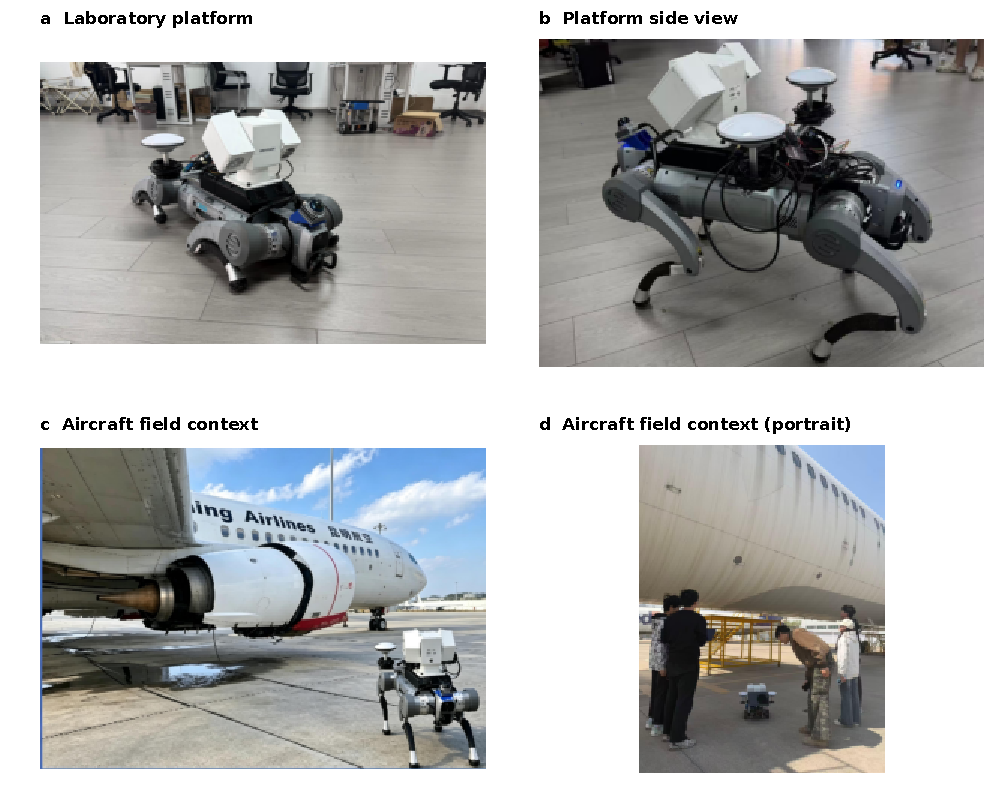
\includegraphics[width=\linewidth]{r8/physical_platforms.pdf}
\caption{All four original platform photographs: laboratory integration, side integration, aircraft field setting and the under-fuselage view. Full original aspect ratios and pixels are retained. These qualitative views do not establish the localization errors or processor latencies measured in the synthetic experiments.}\label{fig:platform}
\end{figure}
\begin{figure}[t]\centering
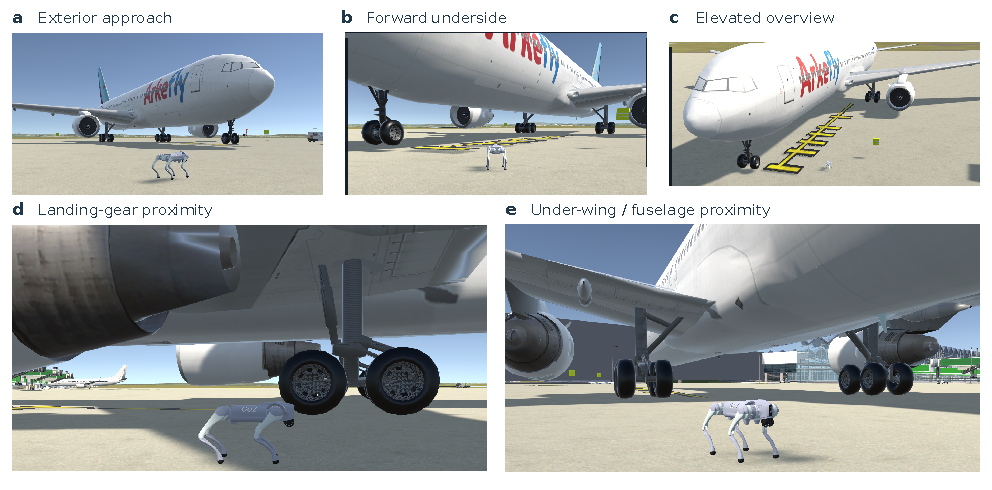
\includegraphics[width=\linewidth]{r6/simulation_views.pdf}
\caption{Simulation views of quadruped aircraft inspection: (a) exterior approach; (b) forward underside; (c) elevated airframe overview; (d) landing-gear proximity; (e) under-wing and fuselage proximity. These five supplied views illustrate deployment geometry. They are shown uncropped, with their original aspect ratios and no pixel retouching. Quantitative localization results use the separately archived geometric sensor and replay inputs.}\label{fig:simulation-scene}
\end{figure}


\section{Experimental results}\label{sec:evaluation}
\subsection{What the contract changes: actions and evidence}
The experiment separates three effects. First, a learned policy changes how much ICP work is executed and when a source version becomes available. Second, requested-event selection chooses one complete calibrated policy before sensing. Third, evidence predicates decide whether its population bound remains applicable to an installed source version. A representation-specific accuracy gain would require a difference from a procedural implementation with the same semantics.

At relaxed and standard services, KG1, CART\_Time and FlatCART have exactly the same stopping, publication and numerical/event outcomes on both confirmation profiles. The full graph and independently validated procedural selector have identical decisions, numerical events and issued receipts on all 32 primary-allowance (0.15) contexts, with 2,048 shared inputs per profile. The 16 primary interval family retains these exact zeros (Fig.~\ref{fig:primary_intervals}). These results attribute the standard-service accuracy improvement to the learned computation policy, rather than to graph storage or inactive constraints.

The time predicate does bind under contention: it changes the CART stopping endpoint on every input in both confirmation profiles. Its shorter execution reduces total work and some observation failures, while increasing integrated trajectory loss. Under the tight service the common hard-budget reservation already stops all compared refinements early, so the additional time predicate changes no endpoint. The declared profile predicate fires for unfitted geometry and larger priors, but adds no numerical change beyond the time/budget controls in this study. Firing a rule and causing a different decision are distinct quantities; all module counts, including these null effects, are retained.
For the nominal confirmation profile, adding time screening changes mean loss by +0.005094~m$^2$s, total work by -3.600~ms and observation failure by -1.660 percentage points. This is a service-dependent trade-off, not uniformly better localization.

For the unfitted confirmation profile, adding time screening changes mean loss by +0.004179~m$^2$s, total work by -3.583~ms and observation failure by -1.904 percentage points. This is a service-dependent trade-off, not uniformly better localization.

\begin{figure}[!htbp]\centering
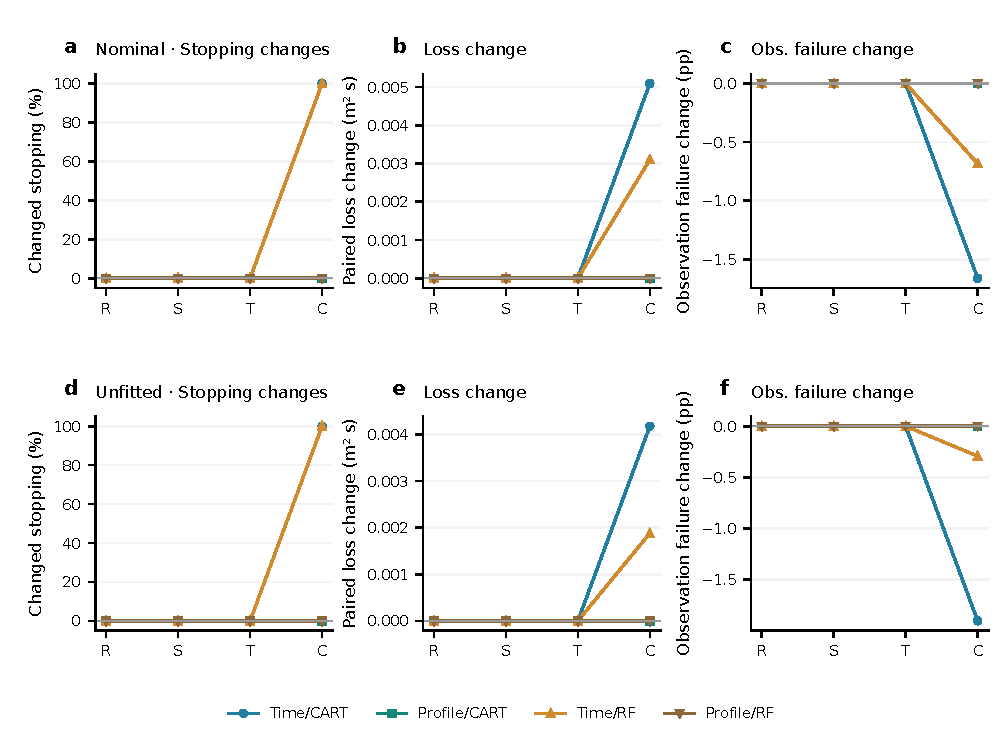
\includegraphics[width=\linewidth]{r8/ablations.pdf}
\caption{Matched numerical-module interventions on all confirmation inputs. R/S/T/C denote relaxed/standard/tight/contended. Time/CART and Time/RF add the same time predicate to their Flat predictors; Profile adds the same declared-profile predicate afterward. Curves are paired descriptive means/counts. Profile effects are zero even where the predicate fires. No source is removed.}\label{fig:ablations}
\end{figure}
Evidence matching and history enforcement act on different outcomes. An incorrect attachment means a violation of the stated applicability protocol; it does not mean that the injected case has experimentally demonstrated population risk above its bound. In the fault fixtures, numerical noninterference can leave risk unchanged while the declared protocol still suspends the statement. Sixteen constructed applicability violations use the actual frozen F1 cards, accompanied by two valid controls including legal rollback. With stripped checks, incorrect attachments number 16; metadata/evidence matching reduces this to four, current-version checking to two, and the source-history latch to zero. The fully validated procedural comparator also has zero incorrect attachments and accepts both valid controls. These are deterministic software cases, not a measured stochastic fault rate or a proof about an arbitrary faulty population. The wider preflight/audits check cold solves, live prefixes, forged payload/checksum combinations, stale dependencies, reconstructed scopes, and rollback. Claims are withdrawn while later valid numerical installation remains available.
\begin{figure}[!htbp]\centering
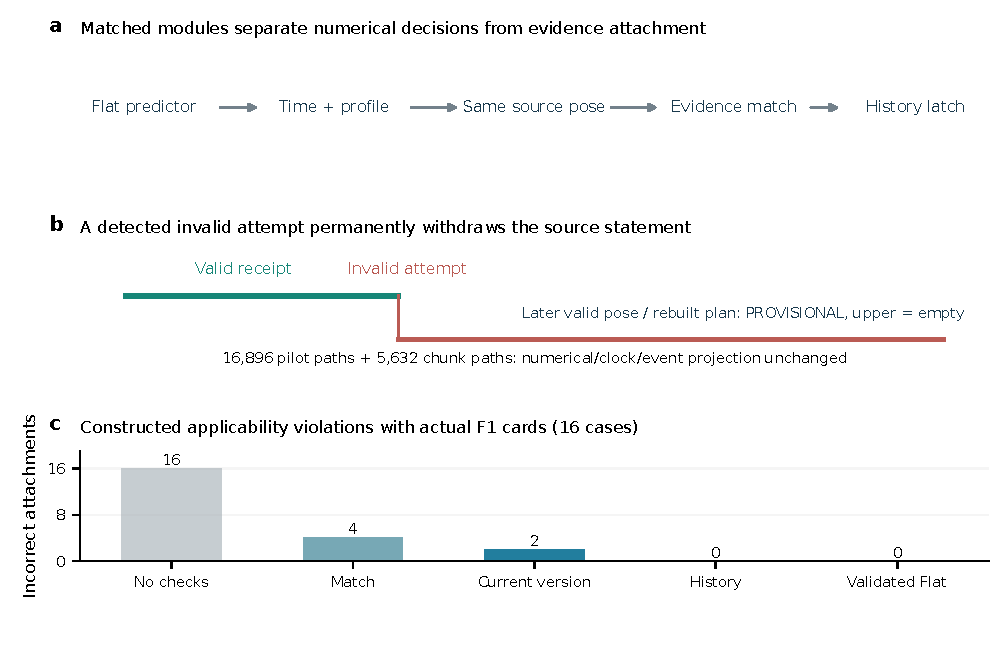
\includegraphics[width=\linewidth]{r8/contract_mechanism.pdf}
\caption{Numerical and applicability mechanisms have different endpoints. (a) Matched prediction/action modules are followed by evidence/lifecycle checks. (b) A detected invalid attempt permanently removes the same source scope\textquotesingle s statement; reconstructed plans do not reset it. (c) Incorrect attachments in 16 constructed invalid cases using real F1 cards. Two normal controls pass every layer. Stripped checks are mechanism ablations; validated Flat is the primary fair competitor. The schematic and exact audit chart were produced by Python code assisted by ChatGPT/Codex (GPT-6).}\label{fig:contract_mechanism}
\end{figure}
\begin{table}[!htbp]\centering\small
\caption{Selective evidence lifetime in excluded software fixtures. One active dependency changes per row; the registry contains the same 528 cards. Counts concern applicability, not new population risk observations. Complete procedural validation can implement the same semantics.}\label{tab:r8-dependencies}
\begin{tabular}{@{}lrr@{}}\toprule
Changed dependency & Revoked cards & Unaffected cards\\\midrule
forecast:rf & 168 & 360\\
artifacts:nominal & 264 & 264\\
event:union & 176 & 352\\
service:standard & 132 & 396\\
clock & 528 & 0\\
\bottomrule\end{tabular}\end{table}
A concrete request chain uses the unfitted profile and standard service at allowance 0.10. The observation request admits ten policies and selects OldRAVC, with $U=0.09994596$; trajectory, both-marginal and union requests are refused. Its margin is only 0.00005404. Thus the task changes evidence eligibility and refusal, not necessarily the selected numerical policy among feasible tasks. The dependency fixtures in Table~\ref{tab:r8-dependencies} make the applicable set traceable to the changed artifact while preserving unrelated cards. Source-version and history checks then govern attachment to the actual installation. These outcomes support inspectable consistency semantics, not a measured maintenance-effort advantage over validated Flat.

\subsection{Same-service localization and the strongest fair control}
Table~\ref{tab:r8-standard} keeps the competitive fixed, learned and old policies under the identical standard service, including shared stage budget and load. The Full rows execute the F1 union-request selection and include actual dispatch/claim overhead; the controlled rows charge the selected executed native prefix plus individually executed components. This component CPU is not the whole-route online CPU reported later.
KG1 reduces loss relative to Fixed2 by 15.68\% in the nominal profile and 12.61\% in the unfitted profile. The corresponding work increases are 16.09\% and 16.07\%. The same predictor without contracts, FlatCART, obtains exactly the same nominal and transfer numerical results. FlatRF/ContractRF largely choose two iterations and remain close to Fixed2. Fixed4 and Final lower mean loss further while paying more work and, in the nominal profile, losing some deadline availability.

\begin{table}[!htbp]\centering\small
\caption{Standard-service confirmation. $L$ is in $10^{-3}$ m$^2$s; $W$ is total modeled work and CPU is measured component CPU (ms/input); failure columns are percentages. Full and validated Flat select FlatCART3 on nominal inputs and OldRAVC on unfitted inputs. Their risk allowance is 0.15 for the direct union. Every row retains all predetermined inputs.}\label{tab:r8-standard}
\begin{tabular}{@{}lrrrrr@{}}\toprule
Method & $L$ & $W$ (ms) & CPU (ms) & Obs. fail & Union fail\\\midrule
\multicolumn{6}{l}{\textit{Nominal, n=2,048}}\\
Fixed2 & 13.833 & 9.221 & 10.498 & 7.18 & 8.64\\
Fixed4 & 11.295 & 12.109 & 13.450 & 6.49 & 7.52\\
Final & 11.295 & 12.109 & 13.463 & 6.49 & 7.52\\
FlatCART & 11.664 & 10.705 & 13.760 & 5.52 & 6.84\\
FlatRF & 13.844 & 9.973 & 12.817 & 7.18 & 8.64\\
ContractRF & 13.844 & 9.973 & 12.764 & 7.18 & 8.64\\
OldRAVC & 12.199 & 9.666 & 11.939 & 5.42 & 6.79\\
KG1 & 11.664 & 10.705 & 13.749 & 5.52 & 6.84\\
Full selector & 12.301 & 9.721 & 10.289 & 5.76 & 7.13\\
Validated Flat & 12.301 & 9.721 & 10.183 & 5.76 & 7.13\\
\multicolumn{6}{l}{\textit{Unfitted, n=2,048}}\\
Fixed2 & 19.938 & 9.220 & 10.525 & 9.08 & 10.06\\
Fixed4 & 17.350 & 11.736 & 13.213 & 8.54 & 9.28\\
Final & 17.350 & 11.736 & 13.174 & 8.54 & 9.28\\
FlatCART & 17.423 & 10.702 & 13.801 & 7.91 & 8.79\\
FlatRF & 19.936 & 9.953 & 12.776 & 9.08 & 10.06\\
ContractRF & 19.936 & 9.953 & 12.733 & 9.08 & 10.06\\
OldRAVC & 17.964 & 9.781 & 11.997 & 8.40 & 9.03\\
KG1 & 17.423 & 10.702 & 13.779 & 7.91 & 8.79\\
Full selector & 17.964 & 9.781 & 10.304 & 8.40 & 9.03\\
Validated Flat & 17.964 & 9.781 & 10.191 & 8.40 & 9.03\\
\bottomrule\end{tabular}\end{table}
\begin{figure}[!htbp]\centering
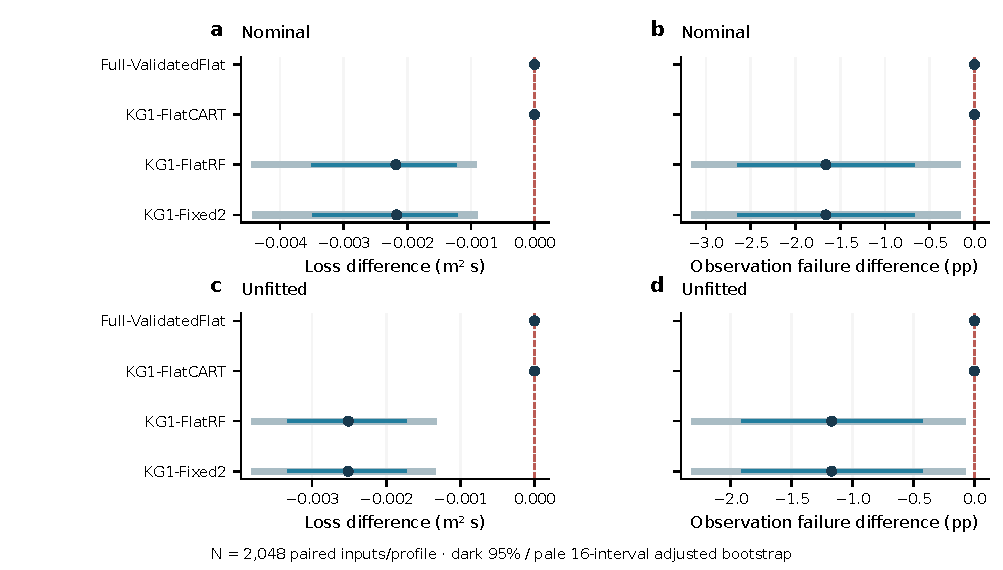
\includegraphics[width=\linewidth]{r8/primary_intervals.pdf}
\caption{All 16 prespecified paired intervals: 2,048 independent confirmation inputs/profile and 32,000 bootstrap replicates. Dark intervals are pointwise 95\%; pale intervals are the 16-interval Bonferroni-adjusted percentile intervals. Exact zero Full--validated Flat and KG1--FlatCART differences remain visible. The intervals are approximate sampling intervals, separate from exact CP calibration.}\label{fig:primary_intervals}
\end{figure}
\begin{figure}[!htbp]\centering
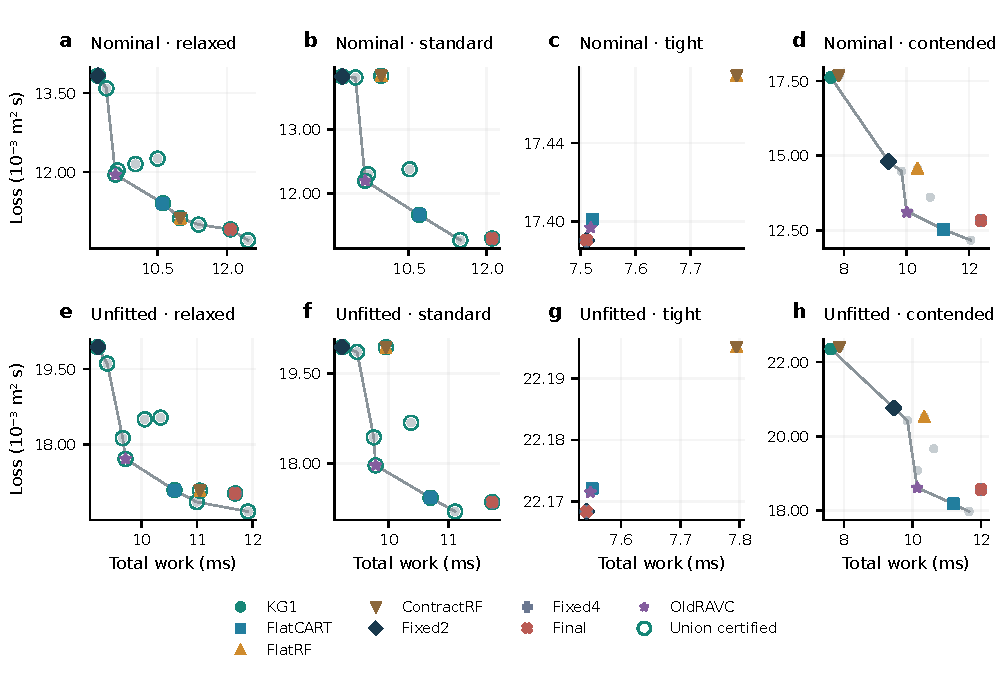
\includegraphics[width=\linewidth]{r8/pareto_services.pdf}
\caption{Work--loss trade-offs across all 22 policies, separately for each confirmation profile/service. Grey points retain the full catalogue, coloured markers identify the principal controls, and open green rings mark policies whose frozen direct-union card has $U\le0.15$. The grey line joins nondominated means; it is descriptive, not a fitted bound or a confidence region. Coincident methods can overlap. The tight service\textquotesingle s common cap explains its small numerical spread.}\label{fig:pareto_services}
\end{figure}
\subsection{Requested events, refusal and actual issued coverage}
The task-aware selector is tested against a competitor that has the same requested events, risk allowance, calibration costs, catalogue and source/history checks. Both produce the same 96 frozen plans. At the primary allowance, 18/32 constructed profile/service/task requests are selected and the remainder refused. This count measures configured catalogue feasibility, not a random field-request success probability.

Relaxed and standard requests admit all four task types. The chosen policy is FlatCART3 for the nominal mixture and OldRAVC for the unfitted mixture. Under contention only the trajectory request is selected; observation, both marginals and direct union are refused. Tight-service requests are all refused. Refusal keeps the source prior, pays its actual monitoring/stream/dispatch costs and counts as observation/union failure. It is not removed from an accuracy denominator. A trajectory-only choice therefore cannot be credited as satisfying an observation request.
\begin{figure}[!htbp]\centering
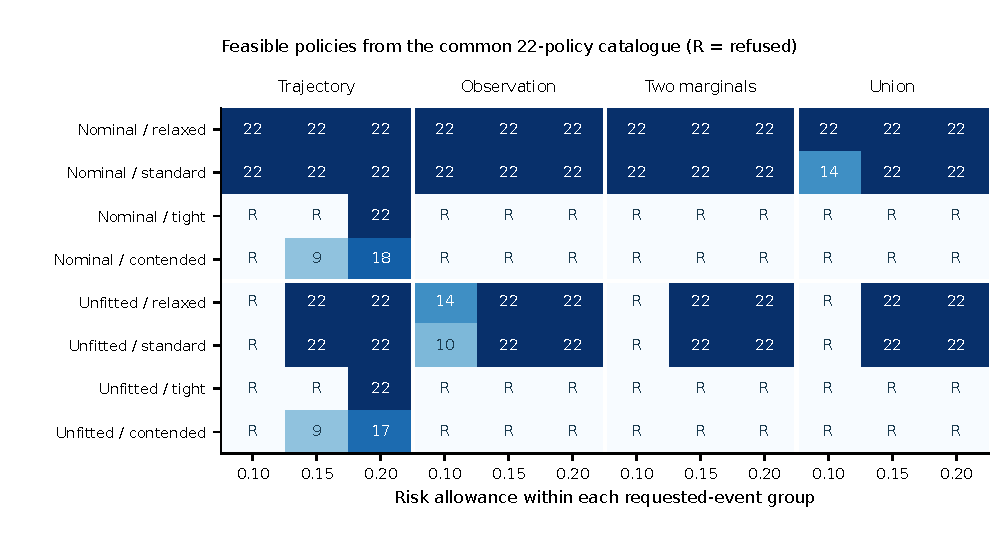
\includegraphics[width=\linewidth]{r8/task_feasibility.pdf}
\caption{All 96 frozen requests: the number of feasible policies in the identical 22-policy catalogue, for four tasks and three allowances. R indicates an empty catalogue. Two marginals request two distinct cards; Union requests its directly calibrated OR event. Full and validated procedural selection have exactly the same feasible sets.}\label{fig:task_feasibility}
\end{figure}
\begin{table}[!htbp]\centering\small
\caption{Selected examples from actual integrated confirmation. Success is a timely positive-version correction with error at most 0.1 m; coverage requires at least one valid issued receipt during execution for each requested event. The same rows hold numerically and for receipts in validated Flat.}\label{tab:r8-task}
\begin{tabular}{@{}llllrr@{}}\toprule
Profile & Service & Task & Policy & Success (\%) & Coverage (\%)\\\midrule
Nominal & standard & union & FlatCART3 & 94.24 & 100.00\\
Nominal & contended & trajectory & FlatCART3 & 49.12 & 100.00\\
Nominal & contended & union & Refused & 0.00 & 0.00\\
Nominal & tight & union & Refused & 0.00 & 0.00\\
Unfitted & standard & union & OldRAVC & 91.60 & 99.95\\
Unfitted & contended & trajectory & OldRAVC & 17.09 & 99.95\\
Unfitted & contended & union & Refused & 0.00 & 0.00\\
Unfitted & tight & union & Refused & 0.00 & 0.00\\
\bottomrule\end{tabular}\end{table}
For selected standard union requests, all nominal sources and 2,047/2,048 unfitted sources issue an applicable receipt. One unfitted source produces no attachable version. A receipt carries a population-event bound and can accompany an inaccurate individual pose; coverage is not scan-conditional safety. Observation success, certification feasibility, receipt coverage and false applicability are accordingly reported separately. Within the canonical confirmation executions the two validators have no receipt discrepancies. The software-fault experiment, rather than this geometric denominator, evaluates malformed applicability.
\subsection{Certificate margins and sensitivity}
Direct union calibration is recomputed on actual trajectory OR observation failures. At standard service, the selected nominal policy has $U_{\cup}=0.085836$ and the selected unfitted policy has $U_{\cup}=0.115254$. Their 0.15 margins are 0.064164 and 0.034746. The unfitted contended trajectory card is more fragile: $U_{\rm tr}=0.146330$, leaving only 0.003670. At allowance 0.10, the standard OldRAVC observation card has only 0.00005404 margin; it does not justify a broad robust-risk claim.

Figures~\ref{fig:certificate_stability} and \ref{fig:certificate_boundary} show that small samples often certify no policy at this family correction, and that feasibility depends on service and confidence. All 28,512 sensitivity rows retain fixed policies and family size; the displayed prefix/confidence grid does not enjoy an extra simultaneous theorem across the diagnostic grid and does not alter F1. The supplement reports every one of the 528 actual cards. Two passing marginals are never interpreted as a passing joint bound. None of the unsupported stress or route profiles receives a transferred episode certificate.
\begin{figure}[!htbp]\centering
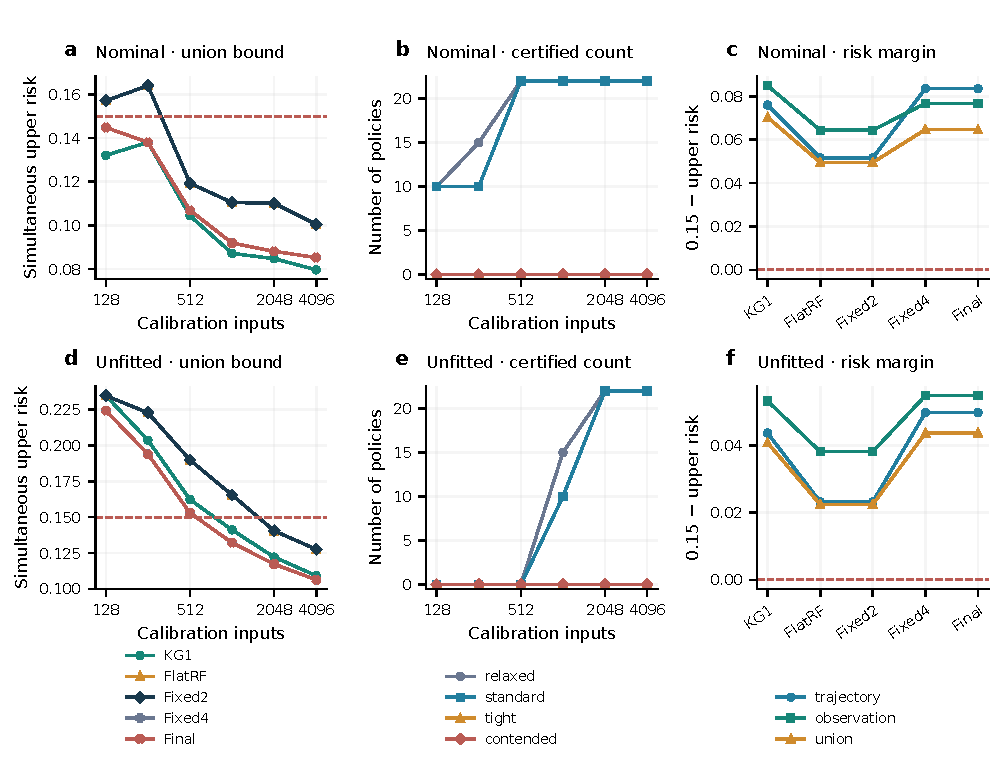
\includegraphics[width=\linewidth]{r8/certificate_stability.pdf}
\caption{Certificate stability under the common 528-member correction. (a,d) Standard direct-union upper bounds versus calibration size. (b,e) The count of union-certified policies by service at allowance 0.15/confidence 0.95. (c,f) Standard full-sample margins for three separately calibrated events. Nested prefixes are descriptive sensitivity; policy selection is not repeated.}\label{fig:certificate_stability}
\end{figure}
\begin{figure}[!htbp]\centering
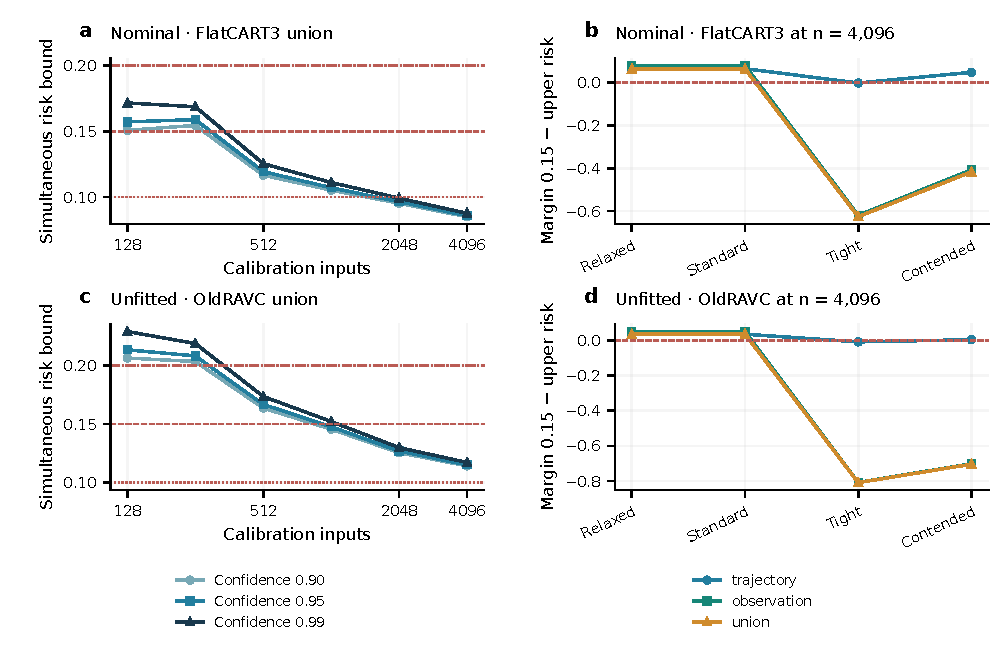
\includegraphics[width=\linewidth]{r8/certificate_boundary.pdf}
\caption{Confidence and failure boundaries for the policies actually chosen at standard service. Left: direct-union bounds at confidence 0.90/0.95/0.99; horizontal reference allowances are 0.10, 0.15 and 0.20. Right: full-sample margins for trajectory, observation and union across the declared services. Negative margins require refusal. The unfitted contended trajectory margin is small even at 4,096 calibration inputs.}\label{fig:certificate_boundary}
\end{figure}
\subsection{Unfitted geometry, stress and concentrated gains}
The held-out geometry results use the original unrefitted predictors but independently matched calibration and confirmation. They demonstrate numerical transfer with fresh evidence; they do not demonstrate zero-shot certification. Unsupported occlusion, degeneracy, prior-shift and map-warp populations remain separate and provisional. Their union failure rates at standard service are retained in Table~\ref{tab:r8-stress}, with complete all-method/service statistics in the release CSVs. A deadline screen cannot repair missing geometric information or a poor map.
\begin{table}[!htbp]\centering\small
\caption{Unsupported stress, n=384 inputs/stratum at standard service. All entries are descriptive with no applicable episode card. Maximum error is the mean of per-episode maxima, in cm; full tail order statistics are in the release CSVs.}\label{tab:r8-stress}
\begin{tabular}{@{}llrrr@{}}\toprule
Stress & Policy & $L$ ($10^{-3}$ m$^2$s) & Union fail (\%) & Mean max (cm)\\\midrule
occlusion & Fixed2 & 19.22 & 24.74 & 6.28\\
occlusion & Final & 17.92 & 23.70 & 5.94\\
occlusion & FlatCART & 17.86 & 22.40 & 6.02\\
occlusion & KG1 & 17.86 & 22.40 & 6.02\\
degeneracy & Fixed2 & 21.29 & 13.02 & 6.21\\
degeneracy & Final & 15.87 & 9.64 & 5.50\\
degeneracy & FlatCART & 17.41 & 11.46 & 5.86\\
degeneracy & KG1 & 17.41 & 11.46 & 5.86\\
prior\_shift & Fixed2 & 27.34 & 20.57 & 7.17\\
prior\_shift & Final & 20.87 & 10.16 & 5.65\\
prior\_shift & FlatCART & 18.78 & 10.68 & 5.84\\
prior\_shift & KG1 & 18.78 & 10.68 & 5.84\\
map\_shift & Fixed2 & 36.43 & 42.19 & 9.31\\
map\_shift & Final & 35.69 & 44.27 & 9.33\\
map\_shift & FlatCART & 35.89 & 43.49 & 9.32\\
map\_shift & KG1 & 35.89 & 43.49 & 9.32\\
\bottomrule\end{tabular}\end{table}
The two largest KG1--Fixed2 contributors account for 27.99\% of the nominal net loss gain. Keeping the remaining 2,046 inputs gives a descriptive mean gain of 0.001563~m$^2$s. The full paired comparison has 442 improved, 374 worsened and 1232 tied inputs; none is deleted from the primary result.

The two largest KG1--Fixed2 contributors account for 10.02\% of the unfitted net loss gain. Keeping the remaining 2,046 inputs gives a descriptive mean gain of 0.002265~m$^2$s. The full paired comparison has 458 improved, 366 worsened and 1224 tied inputs; none is deleted from the primary result.

\begin{figure}[!htbp]\centering
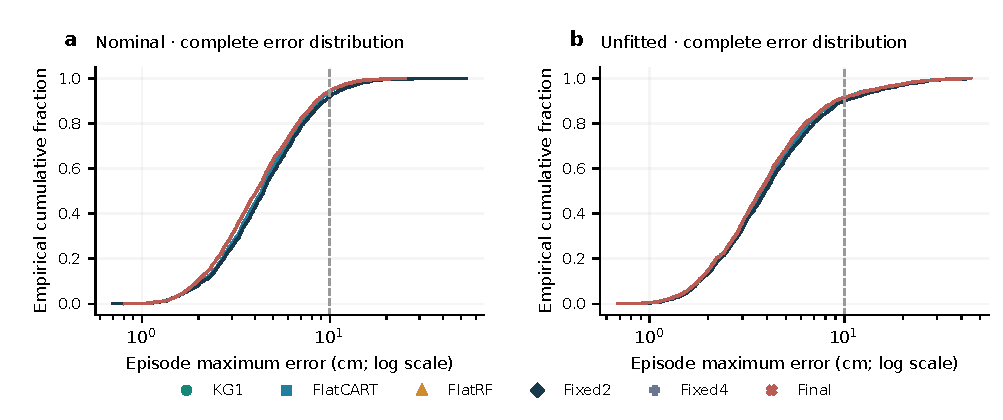
\includegraphics[width=\linewidth]{r8/tail_distributions.pdf}
\caption{Exact empirical cumulative distributions of all 2,048 confirmation episode maxima/profile at standard service; the error axis is logarithmic and the dashed line is 10 cm. Coincident FlatCART/KG1 and FlatRF/Fixed2 curves are retained. Quantiles, worst errors and largest-5\% losses are reported with all observations in the source tables.}\label{fig:tail_distributions}
\end{figure}
\subsection{Complete-route service performance and measured cost}
The 36 new route inputs execute a live estimator rather than reusing independent episode scores. All twelve methods process the same raw scans, measured motion, prior and exogenous load schedule. Figure~\ref{fig:route_frontiers} separates aircraft geometries and ordinary/geometric-stress conditions. The full supplement also includes contention, p95/p99/worst error, failures, readiness, drops, CPU decomposition, work and policy switches.

Fixed2 is an effective ordinary-route choice: it often offers lower CPU, similar or lower error and more timely corrections. Normal routes need only modest refinement, so forecast/dispatch/checking and publication/replay overhead can exceed the gain from adapting a few difficult sources. Geometry and accumulated source errors explain why mean loss improvements on independent episodes do not imply lower long-route RMSE. Contention makes earlier publication useful for deadline readiness, while severe occlusion/map/prior stress produces large error irrespective of source-level authorization.
\begin{table}[!htbp]\centering\small
\caption{Complete-route descriptive means of four matched realizations/geometry/condition, each 600 s and 299 scan opportunities. CPU is directly measured whole-online work, excluding archive access and truth scoring. Full and validated Flat have identical numeric events; their separately measured CPU can differ. No route card is authorized.}\label{tab:r8-route}
\begin{tabular}{@{}lllrrr@{}}\toprule
Geometry & Condition & Method & RMSE (cm) & Success (\%) & CPU (s)\\\midrule
B767 & ordinary & Fixed2 & 3.806 & 97.07 & 2.450\\
B767 & ordinary & KG1 & 3.706 & 96.49 & 2.809\\
B767 & ordinary & Full & 3.715 & 97.24 & 2.514\\
B767 & contention & Fixed2 & 3.555 & 46.99 & 2.322\\
B767 & contention & KG1 & 3.543 & 54.43 & 2.246\\
B767 & contention & Full & 3.531 & 55.02 & 2.019\\
B767 & stress & Fixed2 & 8.185 & 42.22 & 2.154\\
B767 & stress & KG1 & 8.200 & 55.85 & 2.207\\
B767 & stress & Full & 8.158 & 56.19 & 2.300\\
C172 & ordinary & Fixed2 & 4.787 & 94.15 & 2.297\\
C172 & ordinary & KG1 & 4.832 & 93.06 & 2.589\\
C172 & ordinary & Full & 4.805 & 93.81 & 2.518\\
C172 & contention & Fixed2 & 5.237 & 53.01 & 2.121\\
C172 & contention & KG1 & 5.341 & 80.94 & 2.194\\
C172 & contention & Full & 5.234 & 81.61 & 2.028\\
C172 & stress & Fixed2 & 14.488 & 10.20 & 2.168\\
C172 & stress & KG1 & 14.439 & 11.45 & 2.198\\
C172 & stress & Full & 14.414 & 11.20 & 2.221\\
Unfitted & ordinary & Fixed2 & 2.997 & 99.41 & 2.413\\
Unfitted & ordinary & KG1 & 3.018 & 99.25 & 2.618\\
Unfitted & ordinary & Full & 3.006 & 99.25 & 2.395\\
Unfitted & contention & Fixed2 & 3.064 & 39.21 & 2.108\\
Unfitted & contention & KG1 & 2.993 & 43.65 & 2.078\\
Unfitted & contention & Full & 2.994 & 43.65 & 1.975\\
Unfitted & stress & Fixed2 & 9.665 & 38.21 & 2.017\\
Unfitted & stress & KG1 & 9.649 & 46.49 & 2.147\\
Unfitted & stress & Full & 9.663 & 45.74 & 2.211\\
\bottomrule\end{tabular}\end{table}
For C172 contention, KG1's timely-correction success is 80.94\% versus 53.01\% for Fixed2, but its RMSE is 5.341 versus 5.237~cm. This deadline benefit does not imply a mean-accuracy advantage. Full's provisional recommendation yields 81.61\% success and 5.234~cm RMSE, exactly shared by the task-aware procedural selector.

Full and validated Flat first refuse all episode-to-route attachments, then execute the same explicit provisional recommendation. They switch policy 48 times per contention/stress route under the exogenous task/service schedule; ordinary routes use a fixed recommendation. These switches describe an uncertified route service, not adaptive transfer of an episode theorem.

The provider audit recomputes two entire route fixtures with lazy versus prehydrated raw arrays. Every state/error/capture array is bitwise identical, and all non-CPU job/publication/work/events match. The original lazy NPZ access adds archive-decompression CPU inside the timer; the delivered provider moves that offline cost before the frozen online loop and records it separately. Startup is also outside the online timer. Native online costs are host measurements, not embedded latency. Controlled component CPU, inclusive replay including offline assertions/scoring, and full online-route CPU therefore remain separate ledgers.
\begin{figure}[!htbp]\centering
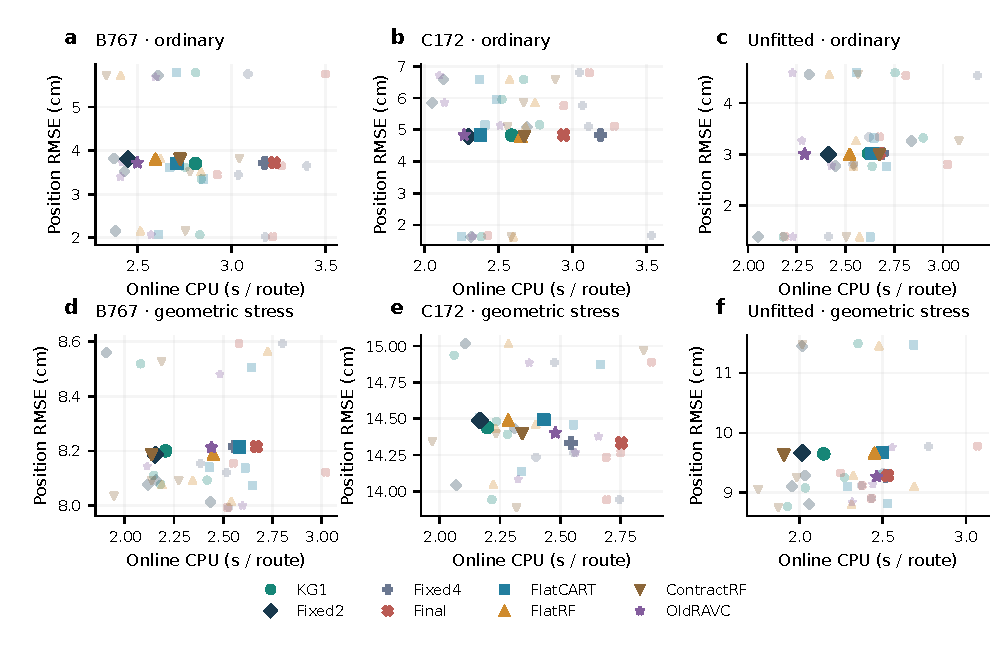
\includegraphics[width=\linewidth]{r8/route_frontiers.pdf}
\caption{Descriptive work--accuracy route frontiers, separated by geometry and condition. Small markers are all four original route realizations; larger markers are their means. Fixed2 and adverse methods remain visible. The CPU boundary covers the entire online loop. The complete twelve-method/three-condition table is retained in the supplement.}\label{fig:route_frontiers}
\end{figure}
\begin{figure}[!htbp]\centering
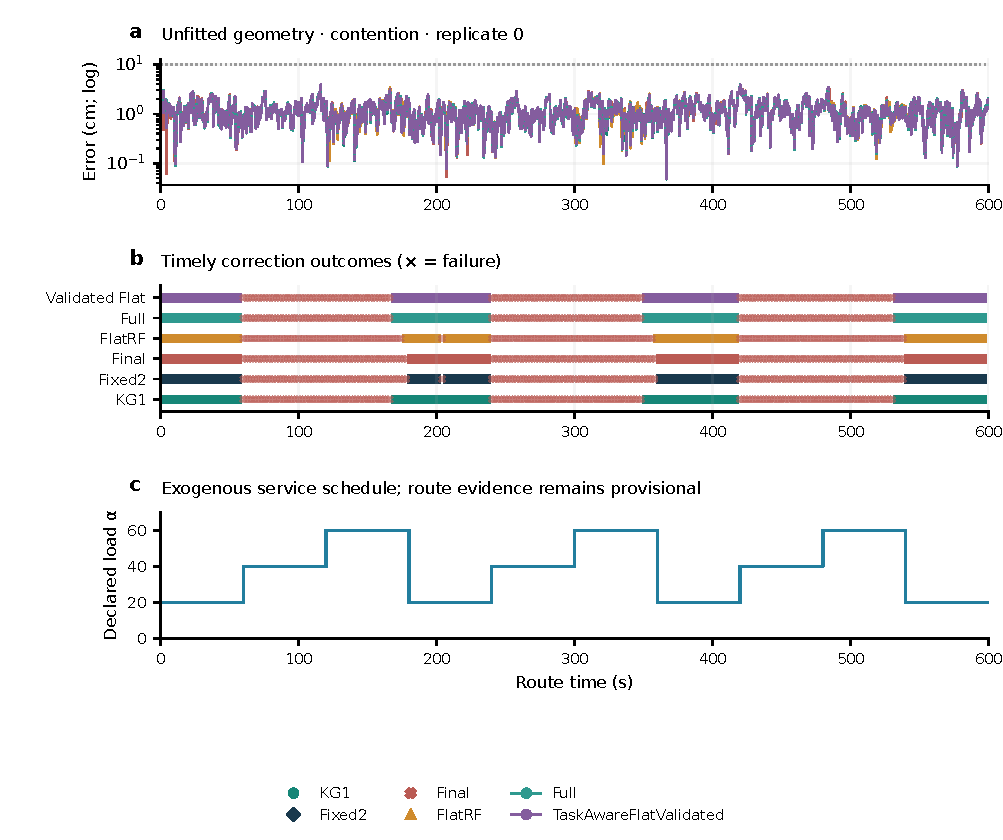
\includegraphics[width=\linewidth]{r8/route_timeseries.pdf}
\caption{The predeclared unfitted-airframe/contention/replicate-zero route. (a) Continuous positional error, including all 6,000 ticks. (b) Timely positive-version correction success at every opportunity; crosses retain failures. (c) The exogenous processor-load schedule. Full and validated Flat traces overlap exactly. Their route recommendations are provisional and have no episode/mission risk bound.}\label{fig:route_timeseries}
\end{figure}


\section{Discussion}\label{sec:discussion}
\subsection{Engineering knowledge contribution and its measured boundary}
The interface turns engineering requirements into executable eligibility, commitment, source execution and evidence-lifetime checks. Its strongest supported contribution is an explicit, testable connection from a task event to the provenance and applicability of its numerical service. It distinguishes a usable late pose from an expired observation statement, a trajectory request from a union request, and a clean later version from a source history that has lost evidence status. Those differences matter to engineering consumers even when pose accuracy does not change.

The fair procedural control is decisive: it reproduces every reported numerical and authorization result. Thus the graph representation is not demonstrated to provide superior numerical decisions, risk bounds or exclusive rejection capability. The matched profile ablation is also redundant in this study. Typed dependency storage provides an inspectable common representation and selective invalidation, but these tests do not establish reduced engineering maintenance effort, operator error or development cost relative to a complete procedural implementation. Such lifecycle/usability outcomes would require their own experiment. The method is a contract-mediated localization/evidence service; it is not a newly demonstrated digital twin or general knowledge-graph reasoning algorithm.

This position also respects prior contract-based anytime control and finite-family risk calibration. Source replacement/replay connects those established ingredients to correlated revisions and event-specific evidence lifetime. The exposure identity explains a possible benefit of early publication; it neither guarantees that every eligible version is better nor eliminates the cost of installation. The current mean-work screen can be optimistic, so direct event calibration applies to the complete actual modeled execution rather than to a predicted deadline.

\subsection{When adaptation is worth its cost}
Relaxed/standard independent episodes reward the CART policy for recognizing some useful refinements. Those gains survive the new confirmation set and top-two influence diagnostic, while coming with more work than Fixed2. Under contention, time screening exchanges integrated loss for earlier availability. The common tight budget makes its additional predicate redundant. Ordinary routes frequently favour Fixed2, because modest difficulty offers little return on learned forecasting and extra publications. Strong map/geometry/prior degradation remains a numerical failure region; refusing an unsupported statement does not fix a pose.

These regions argue for retaining fixed policies inside the task-aware catalogue, not deleting inconvenient controls. The calibration selector may choose an older or Flat policy. Its mean calibration objective can also choose a trade-off that is not optimal on a finite confirmation sample. Simultaneous event bounds justify eligibility under the stated model; they do not prove that the selected policy has minimum true loss or the best hardware deployment cost.

\subsection{Reliability of the evidence}
The new protocol separates development/validation, excluded pilot characterization, calibration, fresh confirmation and unsupported stress. It preserves every seed and counts shared outcomes as paired. Numerical F0, pre-F1 claim amendment, F1 and binding records expose the actual revision chronology. The source-history amendment was made after some calibration execution and before F1; it was limited to attachment semantics, with an explicit projection theorem and conformance audit, rather than concealed as a new initial freeze. Two missing index records were recovered on their original seeds with exact raw-array/file equality. Their recovered CPU metadata is a new measurement. Local manifests are consistency evidence rather than external preregistration or protection from a malicious investigator.

Exact CP statements concern iid complete draws from fixed declared mixtures, conditional on the frozen service clock/predictors/artifacts and ideal simulator random streams. The finite family permits calibration-dependent selection, but the remaining receipt-conditioned subset, individual geometry subgroup and dependent route population have no derived conditional guarantee. Small margins, particularly the contended unfitted trajectory card and the 0.10 observation diagnostic, remain visible. Sensitivity grids are descriptive. Metadata matching certifies neither the physical sampling law nor unknown-distribution detection.

\subsection{Integration and deployment conditions}
The live implementation executes selection, precommit, retained computation, publication, replacement, causal replay and applicability checks. The guarded confirmation driver additionally executes source-history issuance in both implementations. Whole routes refuse transferred evidence and continue explicit provisional service; they do not test a physical feedback controller, online recalibration or a detector of hidden operating changes. Source scopes persist within the trusted registry lifetime; a restart requires restoration or attachment refusal. Producer/code trust, finite payload verification and current-dependency validation are required. Serialized receipt snapshots require consumer revalidation after dependency changes; no remote revocation notification is implemented.

The operation clock is a frozen mean-cost simulation, and the hard sender cap holds only in that normalized model. Added observer CPU is measured, with complete-route online costs separated from inclusive program replay and metadata microbenchmarks. Future physical deployment needs platform-specific service characterization and independent population calibration. The four original photographs and five supplied simulation views preserve engineering context without supplying missing physical performance measurements.


\section{Conclusion}
Executable operating contracts connect engineering task requirements, a frozen localization service and the applicability of its statistical evidence. Source-version replacement and replay support timely numerical updates; event-specific cards, dependency checks and monotone source-history refusal govern statement lifetime. The prospective experiments establish controlled computation trade-offs and integrated applicability behavior while preserving identical results from a fully validated procedural control. Standard-service CART gains are shared by FlatCART, profile constraints add no independent numerical effect here, and ordinary routes can favour Fixed2. Direct union calibration and explicit unsupported-population refusal prevent broader claims than the evidence supplies. The resulting contribution is an inspectable executable interface with reproducible quantitative boundaries. Physical deployment, general lifecycle-effort benefits and stronger representation-specific advantages require additional evidence.

\FloatBarrier
\section*{Evidence and applicability boundary}
The prospective study contains 13,824 distinct synthetic episode inputs: 8,192 calibration, 4,096 confirmation and 1,536 unsupported stress inputs. Forty-eight additional pilot inputs are excluded from inference. Repeated policy, service and task executions add no independent sample size. The 36 complete-route inputs yield 432 executions and carry no episode-to-mission certificate. The operation clock and contention factors are declared simulation services; native CPU ledgers have explicitly different controlled and whole-online-route boundaries. Cards concern unconditional frozen-policy/population events, assume independent source draws and matched deployment distributions, and do not provide scan-conditional risk, OOD detection, physical safety or embedded worst-case timing. The attachment amendment preserves numerical/clock/event traces and withholds statements after detected invalid attempts. Original photographs and supplied simulation images are qualitative context. No new physical robot localization experiment is reported.
\section*{Funding}
This work was supported by the Civil Aviation Safety Capacity Building Fund Project (RJ2025073), ``Pilot-scale development of civil aircraft walk-around inspection and on-wing aero-engine cleaning equipment.''
\section*{Data and code availability}
The reproducibility release contains the frozen prospective protocol, all synthetic input seeds and raw arrays, native solver/predictors, policy and service specifications, calibration/confirmation/stress outcomes, complete route inputs and executions, event cards, attachment-amendment history, execution and asset hashes, analysis and vector-figure scripts, and editable publisher source. Original A19/A20 releases, four original platform photographs, five supplied simulation views and the earlier 2,680-input/81-execution study remain preserved separately. No new physical localization dataset is asserted.
\section*{Declaration of generative AI and AI-assisted technologies}
OpenAI ChatGPT/Codex (GPT-6) assisted research-code development and reconstruction, computational analysis, manuscript drafting and revision, literature organization, and code for exact schematics and data visualizations. Numerical observations were produced by the archived geometric simulation and executed localization code. The authors must review the work and confirm responsibility before submission.
\bibliographystyle{elsarticle-num}
\bibliography{references}
\FloatBarrier
\end{document}
